\chapter{Cross-Firm Information Transfers During Earnings Season: A Network Approach} \label{Chapter:EATE}
\blfootnote{
	This chapter contains material from the following working paper: 
	\nobibliography{thesisbib}
	\begin{itemize}
		\item\bibentry{EA-TE}
	\end{itemize}
}

\section{Introduction}


Major public-firms announce their annual earnings during the first quarter of the year.  The information embedded in these announcements affects the share price of the announcing firm and is incorporated in the share prices of other firms.  Existing literature in finance and accounting focuses on measuring information transfers as effects stemming from firm-specific information releases, such as earnings announcements (see \cite{Foster1981}). This chapter explores how firm information releases influence other firms in the economy without prior assumptions.   We make two simplifying decisions when testing for informational links: an ex-ante source of fundamental linkage between firms, and a time window over which an information transfer will occur.  On the first point, most previous studies assume that links between firms are both persistent and readily observable by a characteristic such as a shared industry (see \cite{Foster1981}) or a customer-supplier relationship (see \cite{OlsenDietrich1985,  AhernHarford2014}).  On the second point, most studies examine an event window, typically several days long, around specific firms' announcements, such as announcing firms in an industry (see \cite{Foster1981, ThomasZhang2008}).

Research by \cite{Billio2012} uses a network approach to examine cross-firm transfers implicit in monthly equity returns for large firms in the financial services sector.  Consistent with a dynamic network of links among these financial firms, these authors find that the extent of cross-firm information transfers increases in recent decades and is associated with significant systemic risk in the financial sector, particularly around the recent 2007-2009 Great Recession.  Evidence presented by \cite{Billio2012} raises the natural question of whether dynamic cross-firm information transfers are present in a broad-based sample of firms and what factors explain variation within this network.

We construct a novel network approach during Q1 2018,  where the network relies on pairwise TE estimates between firms as a proxy for information transfer. Our approach contributes to extant accounting and finance literature.  We provide novel evidence on the network of cross-firm links implied by the lead-lag structure implicit in high-frequency U.S. equity prices observed around releases of earnings information.  By tracing the network of information transfers directly,  we can document several features of cross-firm links that go beyond industry.  Finally,  we use a community detection algorithm to uncover latent clusters of firms with shared information links.  Ultimately we provide evidence that the presence and size of these communities significantly differ depending on the presence of earnings releases.  We hope to encourage future work designed to broaden our understanding of the complex system of information flows inherent in modern equity markets. 

For the remainder of this chapter,  we first discuss the datasets used in this study.   Next, we discuss the methodology for estimating cross-firm information transfers and discuss the network science used to create dynamic cross-firm information transfer networks. We also make observations about the structural properties of the networks.  Then, we conduct an analysis to determine the effect of earnings surprise on dynamic cross-firm information transfers, and we discuss the results of the analysis.  Finally we present an analysis involving community detection within the network of cross-firm transfers and conclude.

\section{Data}
The data in the study comes from Wharton Research Data Services (WRDS) (see \cite{WRDS}). We obtain security prices from the Trade and Quote (TAQ) dataset, which contains all trades and quotes that occurred at a sub-second level.  We use \cite{HoldenJacobsen2014} SAS code to measure the national best bid/offer(NBBO) price. The price is updated as trades or quotes occur.  This means that the timing of the prices is dependent upon when these events occur.  %The NBBO prices are identified from the TAQ dataset and are sampled at particular rates. 

We obtain the NBBO price data for firms in the S\&P 500 in Q1 2018.  We construct ten datasets for each firm at different sampling rates. The sampling rates used in this study are: $1$ second,  $2$ seconds,  $3$ seconds,  $4$ seconds,  $5$ seconds, $10$ seconds,  $15$ seconds,  $30$ seconds,  $60$ seconds,  and $120$ seconds.  For example, at $1$ second sampling rate, there will be 60 NBBO price observations per minute for a particular firm.  CRSP and Compustat are used to obtain firm-specific information.  We also use the Institutional Brokers' Estimate System (IBES) to obtain earnings surprise for firms in the S\&P 500 during Q1 2018.  Throughout the text, we describe how variables are used from IBES, CRSP, and Compustat. 

%Micro structure noise?
% HERE!
\section{Estimating Dynamic Information Transfer Between Firms}

We estimate the amount of information transfer between every unique pair of firms in the S\&P 500 during Q1 2018 (the first 61 days of 2018) by using TE.  To detect information transfer at the minute/sub-minute level between firms in the S\&P 500, we first obtain the NBBO prices from the TAQ data for all firms in the S\&P 500 in Q1 2018.  We create ten datasets from the NBBO data for each date and firm.  We sample the NBBO price data with the following sampling rates: 1,  2,  3,  5,  6,  10,  15,  30,  60,  and 120 seconds. We select these sampling frequencies to allow for a sufficiently large sample of pricing observations in each time window to compute TE.  These sampling frequencies also help determine at what speed information transfer peaks.  

Next for each date,  firm, and sampling rate,  bi-variate TE will be estimated with the NBBO sampled price data using three 130 minute windows throughout the trading day. We use these three windows to determine if there are any consistent information flow patterns during the beginning (9:30am-11:40am), middle (11:40am-1:50pm), or end (1:50pm-4pm) of the trading day.  To summarize TE will be estimated to a specific firm from all other firms in the S\&P 500 for that particular date,  sampling rate,  and interval.  Given that there are 10 sampling rates,  3 windows,  61 days,  and 499 other firms, this amounts to 913,170 TE calculations per firm for Q1 2018 (or 456,585,000 TE calculations in total).  

Data from small sample rates will yield a high number of observations.  %Given that the existing open-source implementations were not suited to estimate bi-variate TE on big data (see Chapter \ref{Chapter:PyIF}) we utilize PyIF (see \cite{PyIF}). 
The 1-second sampling rate has the most observations and is the most costly to estimate TE.  For a particular trading day,   running TE computations with PyIF (see Chapter \ref{Chapter:PyIF}) on the HAL cluster at the National Center for Supercomputing Applications using a single NVIDIA V100 GPU to 1 firm from the other 499 firms for the three windows will take roughly 4 minutes.  For all 500 firms, this took about 2000 minutes.  For all days in Q1 2018, this took about 122,000 minutes (or about 85 days) at the 1-second sampling rate sequentially.  Subsequently, for the 2-second sampling rate, the data is reduced by half. Thus, the wall time was reduced by roughly half.   Given that we can run up to five jobs in parallel on HAL, 1-second TE estimates took 17 days to compute. 

% With PyIF computing TE estimates using the HAL cluster at the National Center for Supercomputing Applications using a single NVIDIA V100 GPU. 

\subsection{Algorithmic Process for Estimating Information Transfer Between firms}

In this section, we outline the algorithmic process to estimate information transfer between firms using the Q1 2018 data (see Algorithm \ref{alg:EstIF}).  In Algorithm \ref{alg:EstIF},  we create a dictionary to map combinations of dates and sampling rates with matrices of computed information transfers.  Given the dates of interest in line 2 and the sampling rates in line 3, we iterate through each date in line 4.  For a particular date, we iterate through each sampling rate in line 5.  For each unique combination of date and sampling rate, we select firms with observations in that date and sampling rate. Next, we create an empty matrix of size Firms\(_i\)\(^2\) by 3, and we use a counter variable to keep track of the observations in line 9. 

Next, we iterate through each firm in the set of firms\(_i\).  In Algorithm \ref{alg:EstIF} the trading day is split into three,  two hour and ten minute windows that represent the beginning (9:30am-11:40am),  middle (11:40am-1:50pm),  and end of the trading day (1:50pm-4pm).  In lines 10-12, we filter the NBBO prices for firm i to the beginning of the trading day,  middle of the trading day, and end of the trading day for a single firm from the set of firm\(_i\) . We repeat this process for all of the firms in the set firm\(_j\) and estimate TE from firm\(_j\) to firm\(_i\).   The TE estimate is assigned to row cnt\(_{ij}\) and column zero of the dateSR\_InfoFlow matrix for the particular key of the dictionary for the TE computation with the morning prices.  Subsequently, the TE estimate is assigned to row cnt\(_{ij}\) and column one or two for the middle of the trading day or end of the trading day, respectively.   Finally, we increment cnt\(_{ij}\) by one and repeat this process for all pair of firms, sampling rates, and days.  Following this algorithm produces a dictionary of computed information transfers for each unique pair of date and sampling rate to perform analyses on.  \\

\begin{algorithm}[H]
\setstretch{1.45}

\SetAlgoLined
%\KwResult{Write here the result }

dateSR\_InfoFlow := \{ \} \;
Dates := All Dates in Q1 2018 \;
SampleRates := [1, 2, 3, 4,  6, 10, 30, 60, 120] secs \;

\For{\(t \in \) Dates}{
	\For{\(SR \in \) SampleRates}{
		Firms\(_i \) := SelectFirms(\(t,SR\)) \;
		Firms\(_j \) := SelectFirms(\(t,SR\)) \;
		dateSR\_InfoFlow[(t,SR)] := Matrix(length(Firms\(_i\))\(^2\), 3) \;
		cnt\(_{ij}\): = 0 \;
		\For{Firm\(_i \in\) Firms\(_i\)}{
			MoPrices\(_i\) := Filter(Firm\(_i\), “9:30am-11:40am”) \;
			MidPrices\(_i\) := Filter(Firm\(_i\), “11:40am-1:50pm”) \;
			AfterPrices\(_i\) := Filter(Firm\(_i\), “1:50pm-4:00pm”) \;	
						
			\For{Firm\(_j \in\) Firms\(_j\)}{
				MoPrices\(_j\) := Filter(Firm\(_j\), “9:30am-11:40am”) \;
				MidPrices\(_j\) := Filter(Firm\(_j\), “11:40am-1:50pm”) \;
				AfterPrices\(_j\) := Filter(Firm\(_j\), “1:50pm-4:00pm”) \;
				
				dateSR\_InfoFlow[(t,SR)] [cnt\(_{ij}\),0] := ComputeTE(MoPrices\(_i\), MoPrices\(_j\)) \;
				dateSR\_InfoFlow[(t,SR)] [cnt\(_{ij}\),1] := ComputeTE(MidPrices\(_i\), MidPrices\(_j\)) \;
				dateSR\_InfoFlow[(t,SR)] [cnt\(_{ij}\),2] := ComputeTE(AfterPrices\(_i\), AfterPrices\(_j\)) \;
				
				cnt\(_{ij}\) += 1
			}
		}
	}
}

\caption{Estimating Information Transfers Between Firms}
\label{alg:EstIF}
\end{algorithm}


\subsection{Network Creation}

After we compute all bi-variate TE estimates, we conduct exploratory data analysis to find patterns or characteristics of the information transfer between firms to explore further.   We employ network analysis techniques (see Chapter \ref{sec:NetworkScience}) to create an information transfer network for all firms at date $t$, sampling rate $s$, and window $w$.  Figure \ref{fig:ExampleNetwork} shows a single network for January 2nd,  2018, during the morning window (9:30am-11:40am).  Each circle in the network is a node that represents a firm. The lines (or edges) between nodes have a thickness determined by the information transfer estimate as computed via transfer entropy. 

The information transfer network in Figure~\ref{fig:ExampleNetwork} has been filtered with a Disparity Filter (see \cite{Serrano}) to reduce the amount of edges in a network.  However, it is still challenging to gather insight from this network.  In addition, there is an information transfer network for each day, $t$,  $s$,  and $w$. Creating networks for all days,  sampling rates, and windows will produce roughly 1,830 networks, which will make it more difficult to discover general insights from the data by viewing them.  An alternative is to look at network measures to gain additional insights from the information transfer networks.

% For all 3 figures roughly 2000 edges are displayed, displaying the full 250,000 connections would yield a network where the ratio of firms to connections is too high to display in this display.  Nevertheless,  representing the data as a network offers an alternative strategy which allows us to compute common network metrics and explore the relationships between firms.

\section{Exploratory Data Analysis}

We now turn to an exploratory analysis of the computed information measures. Figure \ref{fig:TEDist} shows the distribution of information transfers for all days in Q1 2018 for all windows at each sampling rate.   Each subplot is for a particular sample rate,  the x-axis represents the bin value,  and the y-axis represents the percentage of observations in a bin.  Faster sampling rates have lower variance and higher means.  Slower sampling rates have higher variance and smaller means.  A possible explanation is that the frequency of observations decreases due to fewer non-overlapping observations during each 130-minute window.   For example,  there are 7,800 observations per firm at a 1-second sample rate and 130 observations per firm at a 1-minute sample rate. The 1-minute yields fewer data to compute TE and produces a noisier information transfer estimate. 

Table \ref{tab:TEDistIndSampleRate} show additional summary statistics of the information transfers at  each sampling rate.  The 75th and 99th percentile values increase while the median percentile (and lower) values decay as the sample rate becomes slower.  Table \ref{tab:TEMeanWindows} contains the average TE values computed for each of the 130-minute trading windows during the first quarter of 2018 for pairs of firms in the S\&P 500.  

Across sampling rates,  Table \ref{tab:TEMeanWindows} mean values exhibit similar patterns to Table \ref{tab:TEDistIndSampleRate} with a decrease in means as the sampling rates become slower.  Across the three 130-minute windows on each trading day, the 9:30 am-11:40 am (morning) window displays the highest average information transfer.  This latter result is consistent with a surge in trading at the market open each day.

In Table \ref{tab:TEMean30MinWindows},  we investigate the mean TE values at narrower time windows to determine when information transfers tend to peak during the trading day.  Table \ref{tab:TEMean30MinWindows} contains the average TE values computed for thirteen, non-overlapping, thirty-minute trading windows.  Across all sampling rates,  average TE values are highest during the first thirty minutes of the trading day.  Mean TE values then decay throughout the trading day at all sampling rates.  Sampling rates faster than 6 seconds have a slight burst of information transfer within the last hour of the trading day, consistent with information-based trading as part of the daily settlement (closing) trade. 


Table \ref{tab:TEMeanScaledWeightedOutDegree}} shows the average weighted out-degree of the information transfer network at various sampling rates across 61 morning trading periods (9:30am-11:40am).  We scale each degree measure by the number of firms in the network at each measurement period.  Since all firms in the information transfer networks are connected, the average weighted out-degree values across all firms in the first quarter of 2018 are equivalent to the mean weighted in-degree values.  Stated differently, the average of all incoming information transfers from a set of firms to a particular firm is equivalent to the average of all outgoing connections from a set of firms to a firm. The average weighted incoming and outgoing information transfer spikes at a sampling rate of 5 – 6 seconds.


%Given that the Kraskov estimator has a downward bias (see Chapter \ref{IFinFM}) some TE values are slightly below 0.  Figures \ref{fig:20180102-1sec-1of3},  \ref{fig:20180102-1sec-2of3},  and \ref{fig:20180102-1sec-3of3},  show examples of a reduced network on January 2nd 2018 at the 1 second sampling rate between 9:30am-11:40am, 11:40am-1:50pm, and 1:50pm-4pm respectively.   Each of these figures show a portion of the firms in the S\&P 500 and the connections between them, where the firms are the nodes and the connections are the edges with a thickness determined by the value of the transfer entropy estimate.  The highest 0.5\% of edges in the network at these particular times are displayed.  

Tables \ref{tab:TEAutoCorrIn} and \ref{tab:TEAutoCorrOut} present results of ordinary least squares models examining auto-correlation in daily measures of weighted network degree to determine whether firms’ centrality in the network of information transfers displays persistence.  In particular, Table \ref{tab:TEAutoCorrIn} (Table \ref{tab:TEAutoCorrOut}) presents auto-correlations for incoming (outgoing) information transfers based on the weighted in-degree (out-degree) computed from 9:30am-11:40am for each trading day in our 2018 sample period.  The $R^2$ values for both tables exhibit similar behaviors across sampling rates.  In particular, at faster sampling rates we see more explained variation from the morning information transfers with a gradual decay as the sample rates become slower.  The $R^2$ values for the auto-correlation models for outgoing information transfers during morning trading windows in Table \ref{tab:TEAutoCorrOut} are substantially higher than the incoming morning information transfers in Table \ref{tab:TEAutoCorrIn}.  This provides evidence that each firm's position in the information transfer network is persistent. 


\section{Earnings Surprise as a Determinant of Dynamic Information Transfers} % Section with Regression 


Prior literature finds that more informative news events elicit more robust stock price responses among peer firms (see \cite{Foster1981,  Brochet2018}).  Given this,  we examine whether firms with larger absolute earnings surprises (measured relative to the consensus analyst forecast) display stronger information transfers in response to their earnings announcement.  This analysis allows us to shed light on the dynamics of the information transfer network by focusing on variation in the timing of firm’s earnings announcements during earnings season and on variation in the news contained in the announcement.  

In particular,  we estimate an ordinary least squares regression model of the form:

\setlength{\arraycolsep}{0.0em}
\begin{eqnarray}
Y_{iwt} = \alpha + \beta_1 EA_{iwt}  * Morning_{iwt} + \beta_2 EA_{iwt}  * Morning_{iwt} * Abs\_Suprise_{iwt} + \nonumber\\
\beta_3 EA_{iwt}  * Afternoon_{iwt} + \beta_4 EA_{iwt}  * Afternoon_{iwt} * Abs\_Suprise_{iwt} + \nonumber\\
\beta_5 EA_{iwt}  * Evening_{iwt} + \beta_6 EA_{iwt}  * Evening_{iwt} * Abs\_Suprise_{iwt} + \nonumber\\
\beta_7 Share\_Turnover_{it} + \beta_8 Abs\_RET_{it} + \nonumber\\
\beta_9 Morning_{it} + \beta_{10} Evening_{it} + \eta_{i} + \lambda_t +  \epsilon_{i}
\label{eq:EA-Surprise}
\end{eqnarray}
\setlength{\arraycolsep}{1pt}

\noindent \(Y_{iwt}\) is the weighted out-degree (or in-degree) for the \(i^{th}\) firm at the day \(t\) and window \(w\) (i.e, morning, afternoon, or evening).    \(EA_{iwt}\) is an indicator variable for the \(i^{th}\) firm at day \(t\) and window \(w\)  which is set equal to one for trading days with an earnings announcement for the \(i^{th}\) firm made after the prior market close or during the current trading day and to zero otherwise.   \(Morning\),  \(Afternoon\),  and \(Evening\) are indicators variables set equal to one if the current observation is during the 9:30 am - 11:40 am, 11:40 am-1:50 pm,  and 1:50 pm-4:00 pm trading windows, respectively.   

\(Abs\_Surprise\) is the absolute value of the quarterly earnings surprise measured as the difference between actual earnings in I/B/E/S and the last available consensus analyst earnings forecast from the I/B/E/S Summary file,  scaled by the quarter-end stock price available from Compsutat.  The \(Abs\_Surprise\) variable is set to zero for all trading windows other than the first Morning, Afternoon, and Evening trading windows following the announcement.   \(Share\_Turnover\) controls the number of shares traded during the trading day, scaled by the number of shares outstanding on CRSP.  \(Abs\_RET\) and the absolute value of the close-to-close stock return from CRSP.  Equation \ref{eq:EA-Surprise} treats each 130-minute trading window for each firm as a distinct observation.   To focus on within-firm variation in centrality we include firm-fixed effects \(\eta_1\) and trading day fixed-effects \(\lambda_t\). This analysis excludes four outlying observations with absolute earnings surprises larger than 5\% of price. 

We present results of estimating Equation~\ref{eq:EA-Surprise} in Tables~\ref{tab:TEDetOutDeg} and \ref{tab:TEDetInDeg},  where Table \ref{tab:TEDetOutDeg} (Table \ref{tab:TEDetInDeg}) presents results of OLS models where weighted out-degree (in-degree) is the dependent variable.   Results in Table \ref{tab:TEDetOutDeg} show that a firm’s weighted out-degree in the network of information transfers is significantly higher in the trading periods immediately following its earnings announcement when the firm announces a larger earnings surprise. In particular, the positive coefficient on the \(EA*Morning*Abs\_Surprise\) term across the sample rates in models (1) – (10) ranges from 1.672 in model (1) for the 1-second sample rate to 3.117 in model (4) for the 5-second sample rate.  All estimates are statistically significant at a 5\% two-tailed level.  Further, the pattern in coefficients on the \(EA*Morning*Abs\_Surprise\) term across models (1) – (10) in Table \ref{tab:TEDetOutDeg} suggests an information transfer that peaks at 5 seconds, consistent with our transfer entropy estimates presented in Table \ref{tab:TEDistIndSampleRate}.  A significant relation between weighted\_out-degree and earnings news persists into the afternoon trading window at faster sample rates, with significant positive coefficients on the \(EA*Afternoon*Abs\_Surprise\) term for sample rates ranging from 1 second to 3 seconds in models (1) – (3) (two-tailed p-values < 0.05). 

Turning to results in Table \ref{tab:TEDetInDeg} for weighted network in-degree shows that in contrast to results in Table \ref{tab:TEDetOutDeg},  weighted\_in-degree displays limited variation with the magnitude of earnings news released. Except for the \(EA*Morning*Abs\_Surprise\) term in models (1) and (2) for the fastest sample rates, coefficients on the interaction terms with \(Abs\_Surprise\) are generally insignificant at conventional levels and display no clear pattern across sample rates. We interpret these results as suggesting that transfers out to other firms are significant in response to the magnitude of earnings news released, while transfers in are limited in response to the news released.

\section{Community Detection}

We attempt to use community detection algorithms on the information transfer networks to uncover dynamic community formation across morning trading windows.  To limit computational time, we select three morning trading periods for analysis: two periods with a large number of earnings announcements (January 31 and February 1) and one period with no earnings announcements (March 13). We further focus on information transfers at faster speeds by taking the average information transfer across 1 – 6 second sampling rates for each of the three morning trading windows selected and reconstruct the information transfer network.  

In network science literature,  a standard definition of a community is to have more nodes grouped where there is a higher density of edges within a group than between groups.  Given that the information transfer networks are relatively large, we utilize the Clauset-Newman-Moore greedy modularity maximization algorithm to find communities \citep[see][]{Clauset2005}.  While the Clauset-Newman-Moore algorithm aims to find communities in vast networks, it cannot find communities in the information transfer networks. 

The density in our information transfer networks are \(1\), whereas \cite{Clauset2005} benchmark network had a density of \(0.0000125\). Another way to think of this is that the ratio of edges to nodes in our network is 100 times greater than their benchmark network.  While we would ideally employ a community detection algorithm able to scale to the size of these information transfer networks, we are unaware of an such an algorithm.  Thus, we take an alternative approach by reducing the nodes-to-edges ratios for our information transfer networks. This allows us to use standard community detection algorithms.  

With the Clauset-Newman-Moore algorithm to combat the density issue,  we reduce the density (or the node to edges ratio).  We apply a disparity filter (see \cite{Serrano}) to the information transfer networks.  This method locally identifies statistically relevant weighted edges and can filter out relevant connections across all scales of interactions between firms.  This method locally identifies statistically relevant weighted edges by removing any edge that is weaker than a statistical cutoff designed to measure the importance of a given connection to each node.  As a result, the key input for the disparity filter is a researcher-selected value for \(\alpha \) used to identify sufficiently strong connections between nodes

We first take the average information transfer across 1 – 6 second sampling rates for the morning trading windows and reconstruct the information transfer networks.  Next, we apply the disparity filter to find the network backbone, which requires a value for \(\alpha\). The selection of \(\alpha\) is more of an art than science.  Table \ref{tab:backBoneSizes} shows the amount of nodes and edges remaining in a filtered network at a particular  \(\alpha\) value.  A smaller \(\alpha\) will yield an information transfer network that is too sparse to detect communities. A large \(\alpha\) will yield an information transfer network that is too dense to detect communities. 

We select \(\alpha\) based on the Clauset-Newman-Moore algorithm’s ability to detect communities for the most firms in the sample information transfer networks.  We found that when \(\alpha\) = 0.375,  we can detect communities for 100\% of the firms on February 1st and 97\% of the firms on January 31st and March 13th.  We find fewer communities formed during announcement days (January 31st and February 1st) than the trading day with no announcements (March 13th).  However,  most of the community’s sizes during the announcement days are larger than the communities in the March 13th information transfer network (see Figure \ref{fig:NetworkBackboneCommunitySizes}).  On this point,  Figure \ref{fig:NetworkBackboneCommunitySizes} shows that most of the firms in the March 13th information transfer network are in communities with 1, 2, or 3 other firms. During the announcement days, it is less likely to see communities with 1, 2, or 3 other firms; instead, we find more communities with larger sizes.

On the announcement days, the communities typically have only one firm that announced.  There are three cases where a community has two firms that announced and one case where three firms announced. We see a diverse set of industries connected within and across the detected communities.   Figure \ref{fig:Community20180313full} presents the full set of nodes and resulting communities for the information transfer network for the March 13th morning trading window. This figure shows the presence of several larger communities with a handful of central (larger) nodes. In addition, Figure \ref{fig:Community20180313full} shows a number of firms (in gray) appearing with small (or no) communities.   To aid in graphically presenting these communities, Figures \ref{fig:Community20180131},  \ref{fig:Community20180201}, and \ref{fig:Community20180313}  presents only communities with at least 9 firms in the resulting community.  

For all the information transfer networks, there is a dynamic formation of hubs.  Some hubs reoccur, and others form during a particular trading day.   For example,  in Figures \ref{fig:Community20180131},  \ref{fig:Community20180201}, and \ref{fig:Community20180313} Amazon (AMZN), National Weather Service (NWS), and Mettler-Toledo International Inc (MTD) are hubs during the announcement days and the non-announcement day despite the different connections that form to each of these hubs.  However, when Boeing (BA) announced on January 31st, it temporarily appears as a hub in Figure~\ref{fig:Community20180131} for that morning information transfer network. The networks' characteristics provide evidence that the networks are not random, which indicates that we are capturing valid cross-firm information transfers via our measurement of transfer entropies. 


\section{Conclusion}

We introduce a new approach to examine information transfers around earnings season.  We study the network effect of earnings announcements by constructing daily networks of pairwise cross-firm information transfers.  Our approach to construct these networks relies on non-parametric estimates in equity prices with measures of transfer entropy drawn from information theory.  While it is known that earnings information produced by a single firm is incorporated into the firm's equity price,  we provide evidence that this information flows to the equity prices of other firms across industries.  In particular our tests show that cross-firm links are substantially stronger for firms on days with releases of earnings information and firms with more unexpected earnings news, consistent with the network of cross-firm information transfers dynamically responding to shifts in the information landscape.  Further,  we find that communities form between firms with links that are not adequately captured by characteristics that are the focus of existing literature.  These analyses also demonstrate that the prior literature’s focus on measuring information connections between firms in the same industry or along the supply chain likely result in missing important information linkages across more diverse firms. 


%Future work?

%Communtity detection algorithm for denser network


\newpage
\section{Figures and Tables}
%\subsection{Figures}

\rotatebox{90}{\begin{minipage}{0.9\textheight}
   \centerline{ 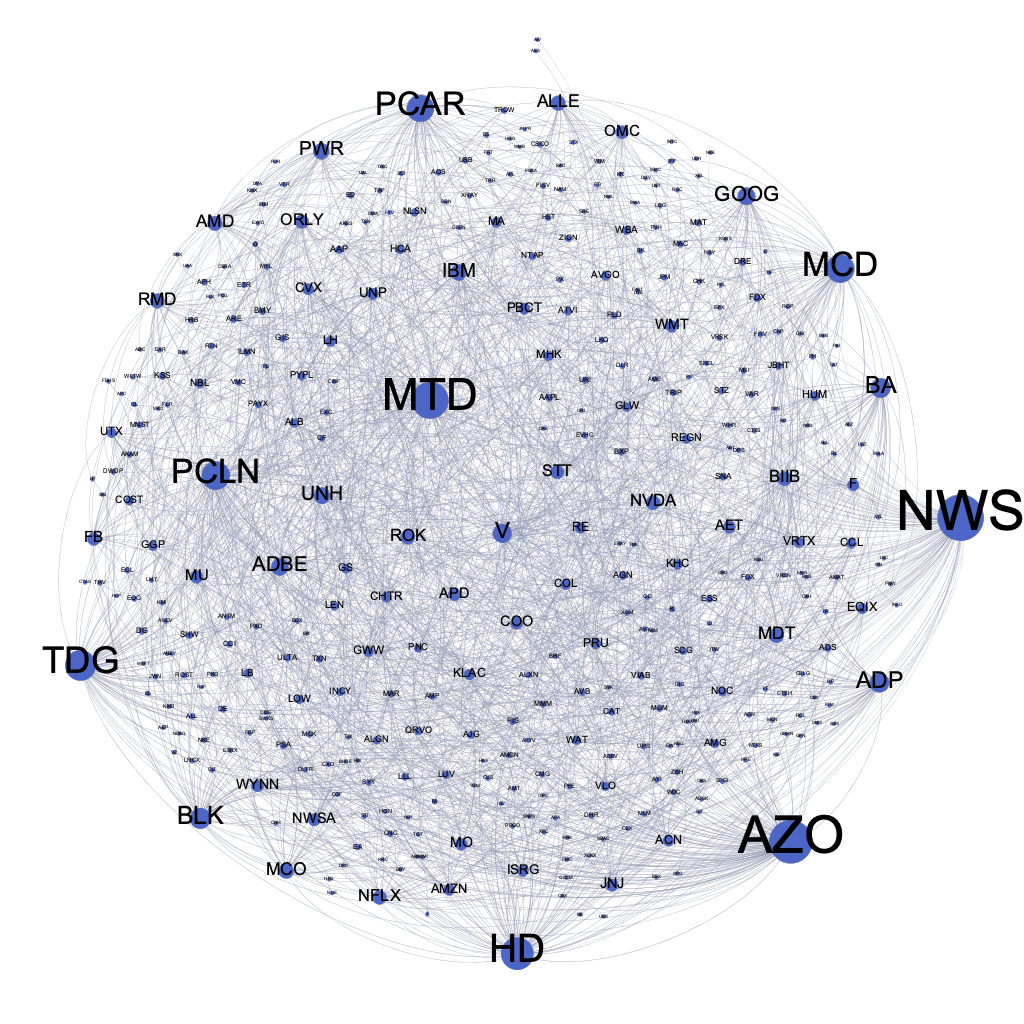
\includegraphics[width=0.7\textwidth]{figures/EarnAnnounceTE/ExampleNetwork-Jan2nd.png}}
    \captionof{figure}{This figure shows an example network on January 2nd during the morning window (9:30 am-11:40 am) at the 1-second sampling rate.}
  \label{fig:ExampleNetwork}
\end{minipage}}



%\begin{figure}[htb!]
%  \centerline{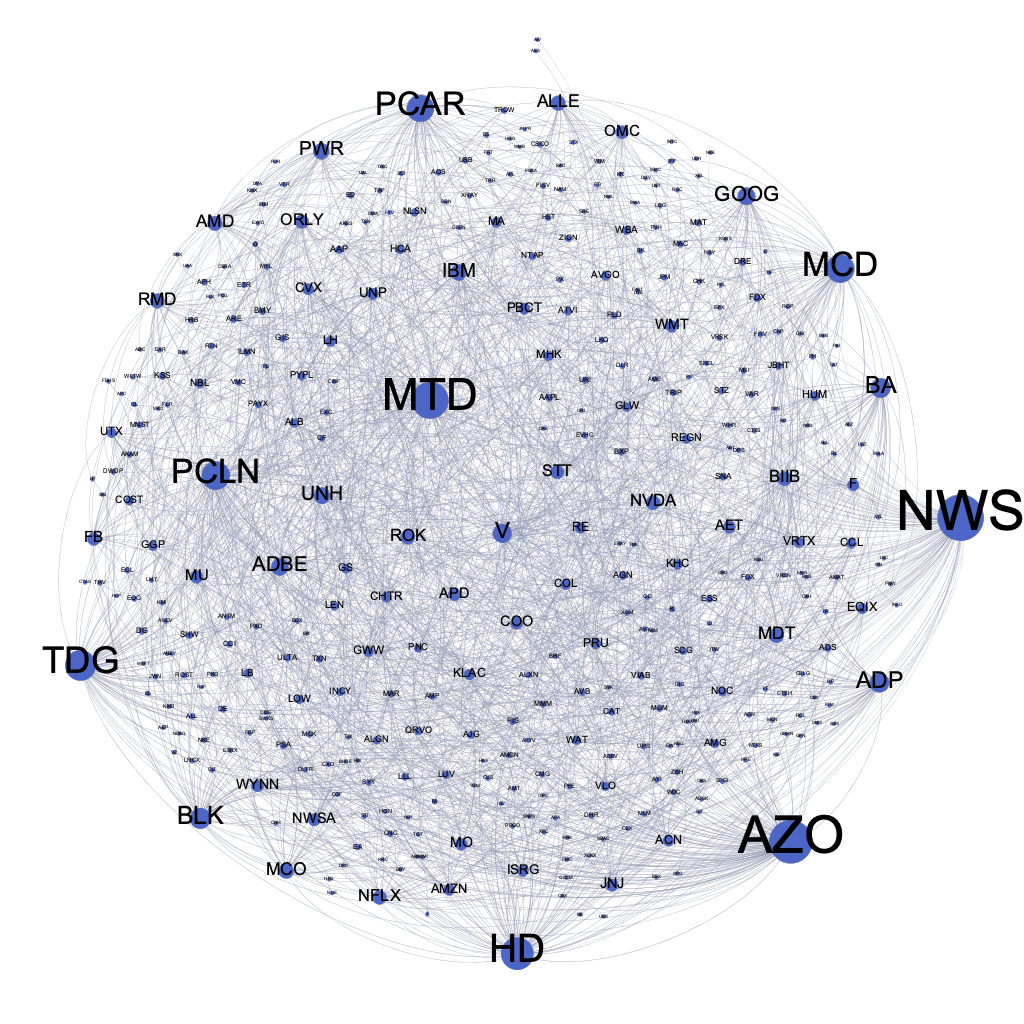
\includegraphics[scale=0.45]{figures/EarnAnnounceTE/ExampleNetwork-Jan2nd.png}}
%  \caption{This figure shows an example network on January 2nd during the morning window (9:30 am-11:40 am) at the 1-second sampling rate.}
%  \label{fig:ExampleNetwork}
%\end{figure}

\begin{figure}[htb!]
  \centerline{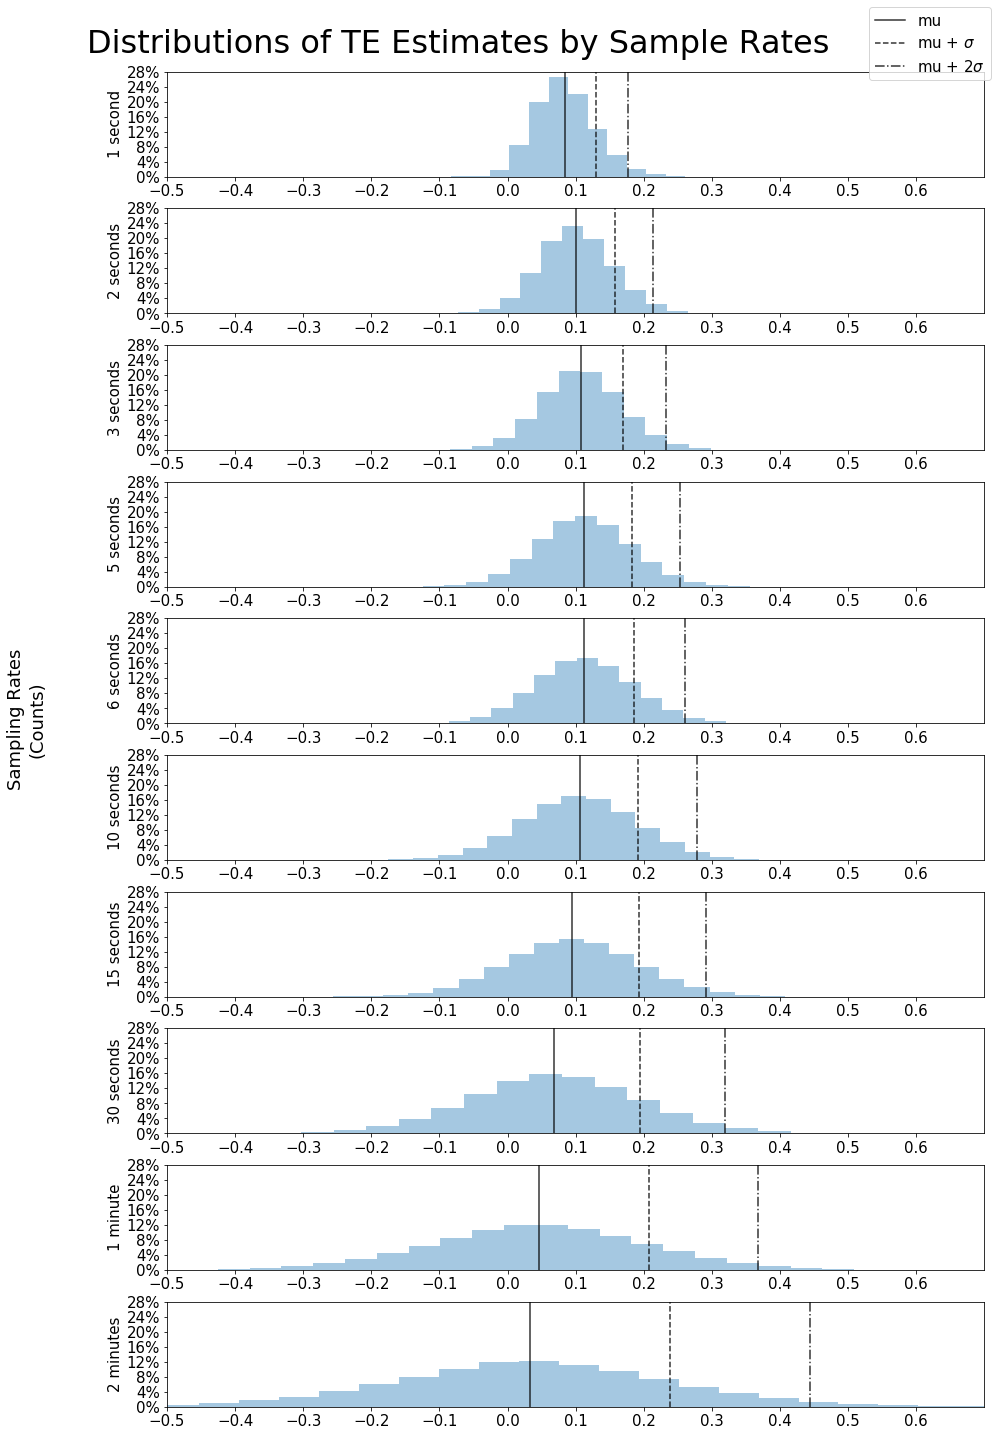
\includegraphics[scale=0.4]{figures/EarnAnnounceTE/TEDist.png}}
  \caption{This figure shows the distributions of information transfers between firms during Q1 2018 for all sampling rates.}
  \label{fig:TEDist}
\end{figure}

\begin{sidewaysfigure}[htb!]
  \centerline{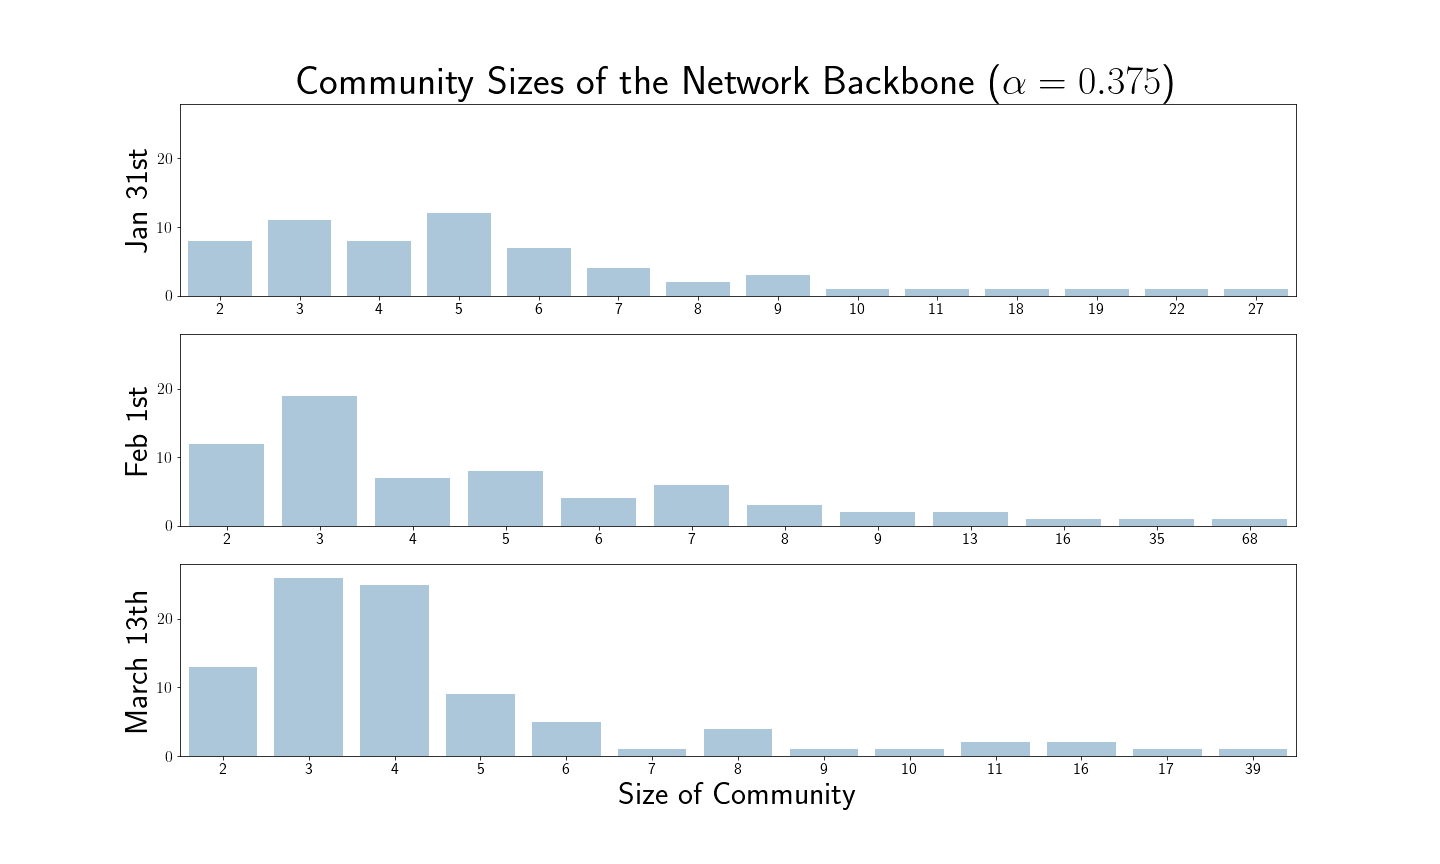
\includegraphics[scale=0.4]{figures/EarnAnnounceTE/NetworkBackboneCommunitySizes.png}}
  \caption{Community sizes of the network backbone when $\alpha=0.375$ for January 31st,  February 1st,  and March 13th}
  \label{fig:NetworkBackboneCommunitySizes}
\end{sidewaysfigure}

% Communtity Detection

\begin{figure}[htb!]
  \centerline{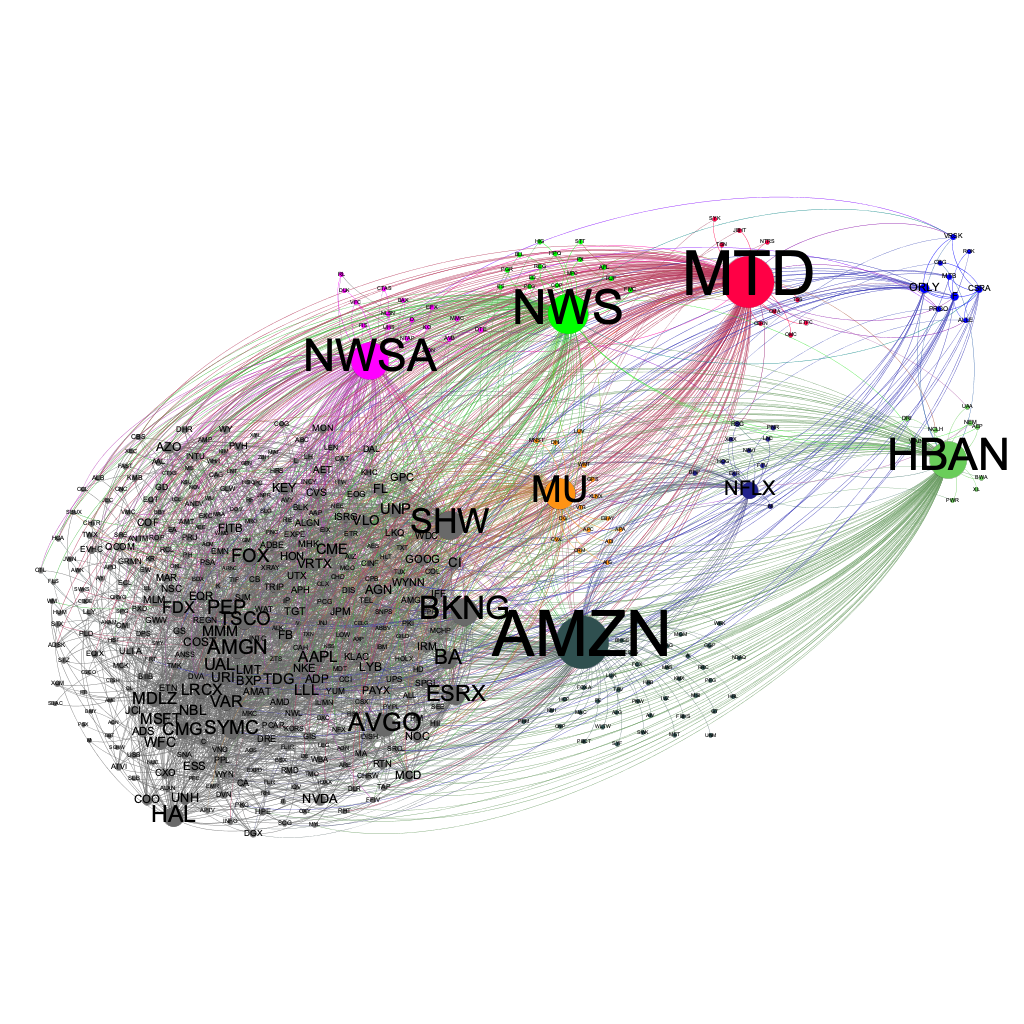
\includegraphics[scale=0.5]{figures/EarnAnnounceTE/20180313mt-8colored-curved}}
  \caption{This figure shows the backbone network displaying communities for March 13th.  Each color represents a specific community, and the node's size represents the degree of the node.  All communities and nodes with at least 9 firms appear with a color other than gray for each community. }
  \label{fig:Community20180313full}
\end{figure}


\begin{figure}[htb!]
  \centerline{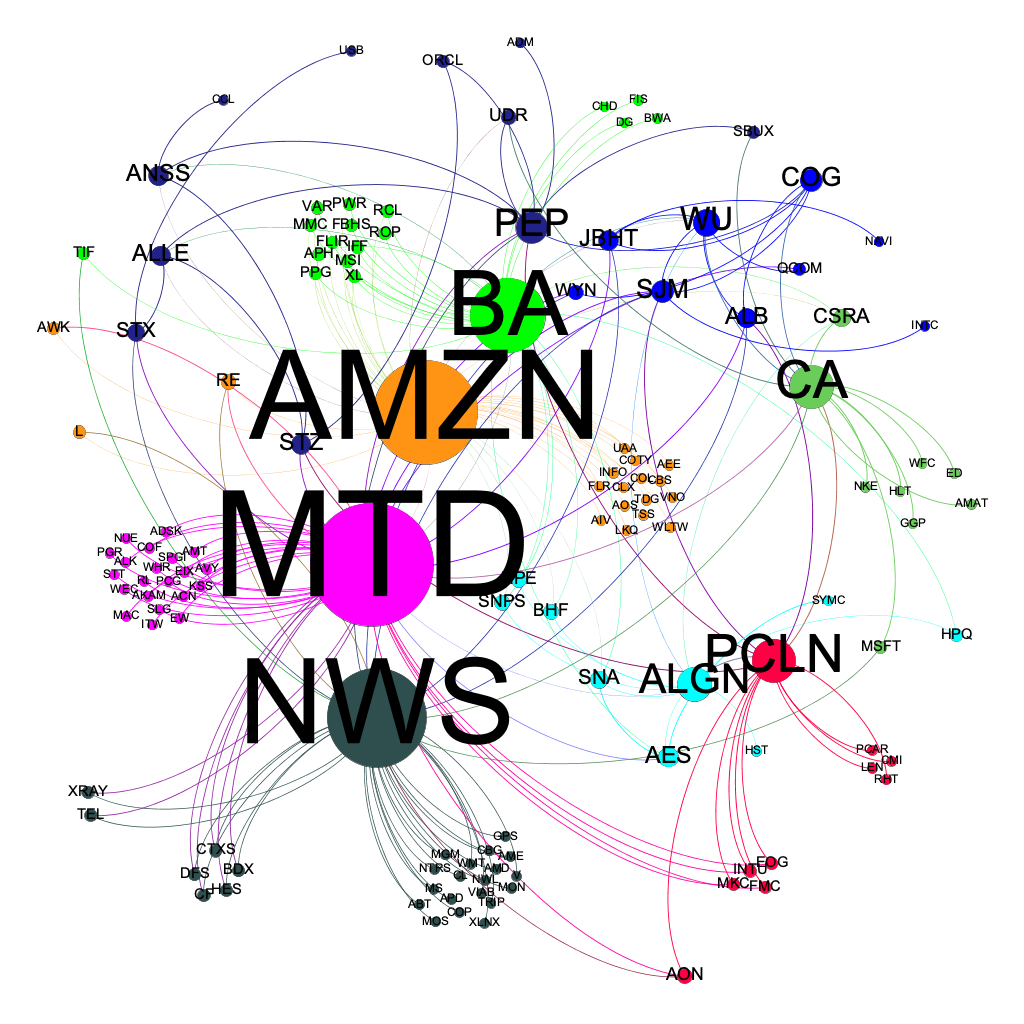
\includegraphics[scale=0.5]{figures/EarnAnnounceTE/20180131OnlyC-curved.png}}
  \caption{This figure shows the backbone network displaying communities for January 31st, where at least nine firms are in the community.  Each color represents a specific community, and the node's size represents the degree of the node.}
  \label{fig:Community20180131}
\end{figure}

\begin{figure}[htb!]
  \centerline{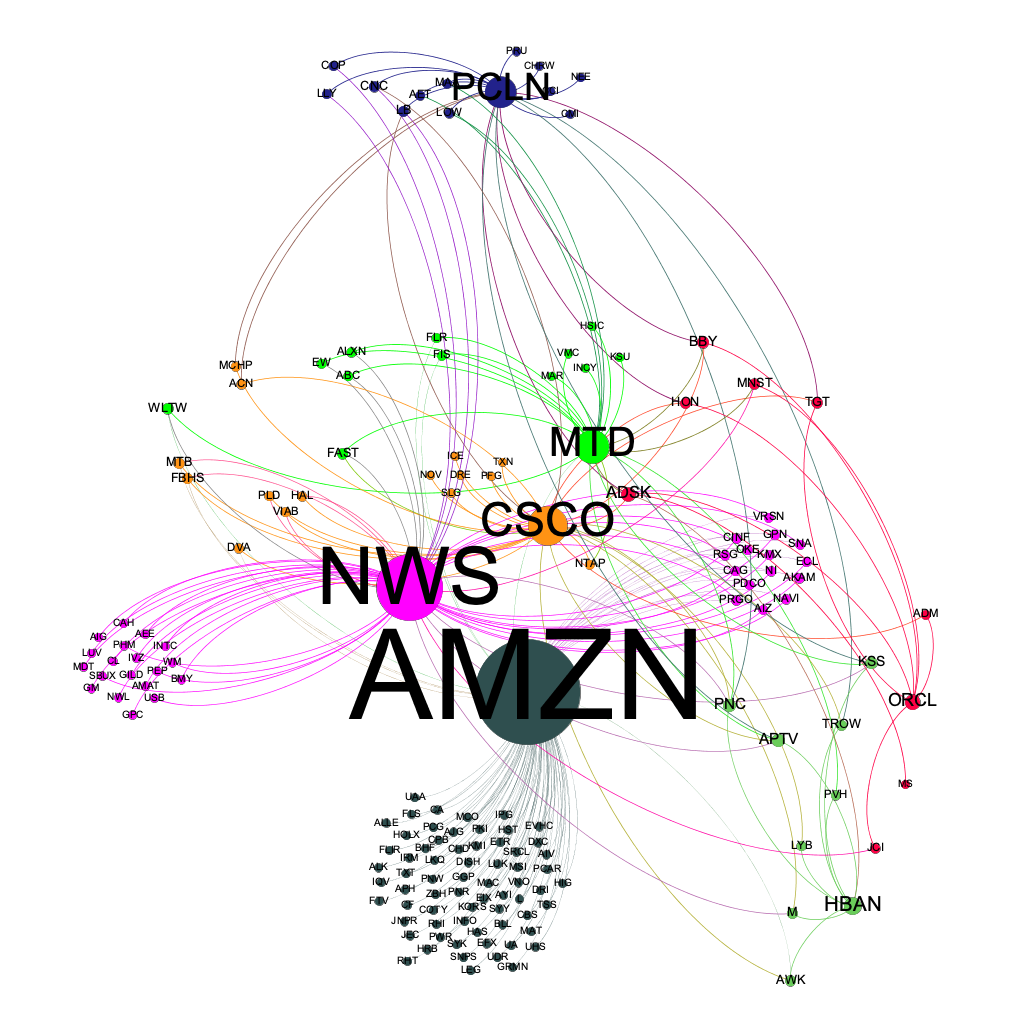
\includegraphics[scale=0.5]{figures/EarnAnnounceTE/20180201OnlyC-curved.png}}
  \caption{This figure shows the backbone network displaying communities for February 1st, where at least nine firms are in the community.  Each color represents a specific community, and the node's size represents the degree of the node.}
  \label{fig:Community20180201}
\end{figure}

\begin{figure}[htb!]
  \centerline{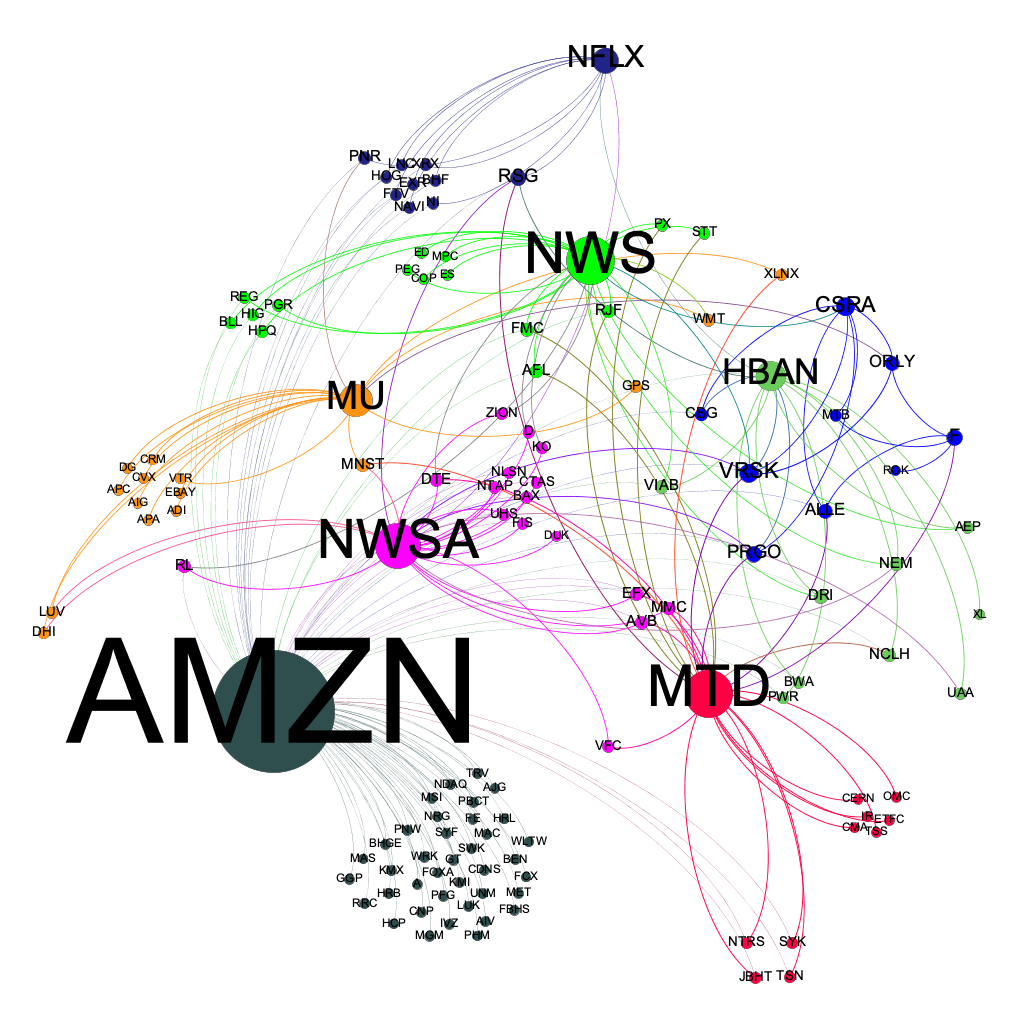
\includegraphics[scale=0.5]{figures/EarnAnnounceTE/20180313OnlyC-curved.png}}
  \caption{This figure shows the backbone network displaying communities for March 13th where at least nine firms are in the community.  Each color represents a specific community, and the node's size represents the degree of the node.}
  \label{fig:Community20180313}
\end{figure}



\clearpage

\begin{sidewaystable*}[htb!]
\centering
\resizebox{\columnwidth}{!}{
\begin{tabular}{|l|c|c|c|c|c|c|c|c|c|c|}
\hline
\multicolumn{1}{|r|}{\textbf{Sample Rate}} & \textbf{1 second} & \textbf{2 seconds} & \textbf{3 seconds} & \textbf{5 seconds} & \textbf{6 seconds} & \textbf{10 seconds} & \textbf{15 seconds} & \textbf{30 seconds} & \textbf{1 minute} & \textbf{2 minutes} \\ \hline
\textbf{Mean}                              & 0.084             & 0.101              & 0.108              & 0.112              & 0.112              & 0.106               & 0.094               & 0.069               & 0.046             & 0.033              \\ \hline
\textbf{St. Deviation}                     & 0.046             & 0.056              & 0.062              & 0.070              & 0.074              & 0.086               & 0.099               & 0.125               & 0.161             & 0.206              \\ \hline
\textbf{1st percentile}                    & -0.014            & -0.025             & -0.033             & -0.052             & -0.061             & -0.099              & -0.141              & -0.233              & -0.344            & -0.472             \\ \hline
\textbf{Q1}                                & 0.054             & 0.065              & 0.069              & 0.067              & 0.064              & 0.049               & 0.030               & -0.013              & -0.058            & -0.098             \\ \hline
\textbf{Median}                            & 0.082             & 0.100              & 0.108              & 0.112              & 0.112              & 0.106               & 0.094               & 0.069               & 0.047             & 0.034              \\ \hline
\textbf{Q3}                                & 0.112             & 0.136              & 0.148              & 0.158              & 0.160              & 0.163               & 0.159               & 0.152               & 0.153             & 0.167              \\ \hline
\textbf{99th percentile}                   & 0.201             & 0.234              & 0.253              & 0.275              & 0.283              & 0.306               & 0.323               & 0.359               & 0.422             & 0.517              \\ \hline
\end{tabular}
}
\caption{This table shows the summary statistics for transfer entropy estimates during non-overlapping 130-minute trading windows. }
\label{tab:TEDistIndSampleRate}
\end{sidewaystable*}


\begin{sidewaystable*}[htb!]
\centering
\resizebox{\columnwidth}{!}{
\begin{tabular}{|c|c|c|c|c|c|c|c|c|c|c|}
\hline
\multicolumn{1}{|r|}{\textbf{Sample Rate}} & \textbf{1 second} & \textbf{2 seconds} & \textbf{3 seconds} & \textbf{5 seconds} & \textbf{6 seconds} & \textbf{10 seconds} & \textbf{15 seconds} & \textbf{30 seconds} & \textbf{1 minute} & \textbf{2 minutes} \\ \hline
\textbf{9:30am-11:40am}                    & 0.097             & 0.117              & 0.125              & 0.130              & 0.130              & 0.123               & 0.109               & 0.082               & 0.058             & 0.044              \\ \hline
\textbf{11:40am-1:50pm}                    & 0.071             & 0.088              & 0.096              & 0.102              & 0.103              & 0.100               & 0.091               & 0.067               & 0.044             & 0.030              \\ \hline
\textbf{1:50pm-4pm}                        & 0.083             & 0.098              & 0.103              & 0.105              & 0.103              & 0.095               & 0.082               & 0.057               & 0.037             & 0.024              \\ \hline
\end{tabular}
}
\caption{Mean transfer entropy estimates for non-overlapping 130-minute daily trading windows at each sample rate.}
\label{tab:TEMeanWindows}
\end{sidewaystable*}

\begin{sidewaystable*}[htb!]
\centering
\resizebox{\columnwidth}{!}{
\begin{tabular}{|c|c|c|c|c|c|c|c|c|}
\hline
\multicolumn{1}{|r|}{\textbf{Sample Rate}} & \textbf{1 second} & \textbf{2 seconds} & \textbf{3 seconds} & \textbf{5 seconds} & \textbf{6 seconds} & \textbf{10 seconds} & \textbf{15 seconds} & \textbf{30 seconds} \\ \hline
\textbf{09:30AM-10:00AM}                   & 0.099             & 0.118              & 0.127              & 0.130              & 0.129              & 0.118               & 0.105               & 0.078               \\ \hline
\textbf{10:00AM-10:30AM}                   & 0.085             & 0.101              & 0.107              & 0.109              & 0.108              & 0.098               & 0.084               & 0.058               \\ \hline
\textbf{10:30AM-11:00AM}                   & 0.077             & 0.093              & 0.099              & 0.101              & 0.100              & 0.092               & 0.082               & 0.058               \\ \hline
\textbf{11:00AM-11:30AM}                   & 0.073             & 0.087              & 0.093              & 0.096              & 0.095              & 0.089               & 0.077               & 0.056               \\ \hline
\textbf{11:30AM-12:00PM}                   & 0.069             & 0.085              & 0.091              & 0.095              & 0.095              & 0.090               & 0.080               & 0.059               \\ \hline
\textbf{12:00PM-12:30PM}                   & 0.065             & 0.080              & 0.086              & 0.091              & 0.091              & 0.087               & 0.080               & 0.058               \\ \hline
\textbf{12:30PM-01:00PM}                   & 0.061             & 0.076              & 0.084              & 0.089              & 0.089              & 0.086               & 0.078               & 0.057               \\ \hline
\textbf{01:00PM-01:30PM}                   & 0.061             & 0.076              & 0.082              & 0.086              & 0.088              & 0.085               & 0.076               & 0.057               \\ \hline
\textbf{01:30PM-02:00PM}                   & 0.062             & 0.076              & 0.083              & 0.088              & 0.089              & 0.085               & 0.076               & 0.058               \\ \hline
\textbf{02:00PM-02:30PM}                   & 0.067             & 0.081              & 0.087              & 0.091              & 0.091              & 0.085               & 0.076               & 0.053               \\ \hline
\textbf{02:30PM-03:00PM}                   & 0.066             & 0.079              & 0.086              & 0.089              & 0.088              & 0.082               & 0.072               & 0.052               \\ \hline
\textbf{03:00PM-03:30PM}                   & 0.072             & 0.084              & 0.090              & 0.090              & 0.088              & 0.079               & 0.067               & 0.043               \\ \hline
\textbf{03:30PM-04:00PM}                   & 0.087             & 0.093              & 0.091              & 0.084              & 0.080              & 0.067               & 0.055               & 0.041               \\ \hline
\end{tabular}}
\caption{Mean transfer entropy estimates for non-overlapping 30-minute daily trading windows at each sample rate.}
\label{tab:TEMean30MinWindows}
\end{sidewaystable*}

\begin{sidewaystable*}[htb!]
\centering
\resizebox{\columnwidth}{!}{
\begin{tabular}{r|c|c|c|c|c|c|c|c|c|c|}
\cline{2-11}
\multicolumn{1}{l|}{}      & 1 SECOND & 2 SECONDS & 3 SECONDS & 5 SECONDS & 6 SECONDS & 10 SECONDS & 15 SECONDS & 30 SECONDS & 1 MINUTE & 2 MINUTES \\ \hline
\multicolumn{1}{|c|}{MEAN} & 0.253    & 0.305     & 0.328     & 0.341     & 0.342     & 0.331      & 0.309      & 0.273      & 0.268    & 0.294     \\ \hline
\multicolumn{1}{|c|}{STD}  & 0.037    & 0.031     & 0.024     & 0.015     & 0.014     & 0.020      & 0.027      & 0.033      & 0.030    & 0.026     \\ \hline
\multicolumn{1}{|c|}{MIN}  & 0.205    & 0.260     & 0.291     & 0.317     & 0.312     & 0.271      & 0.227      & 0.193      & 0.200    & 0.235     \\ \hline
\multicolumn{1}{|c|}{1\%}  & 0.207    & 0.260     & 0.294     & 0.318     & 0.315     & 0.272      & 0.233      & 0.200      & 0.201    & 0.239     \\ \hline
\multicolumn{1}{|c|}{25\%} & 0.224    & 0.281     & 0.309     & 0.330     & 0.332     & 0.323      & 0.296      & 0.257      & 0.250    & 0.278     \\ \hline
\multicolumn{1}{|c|}{50\%} & 0.251    & 0.302     & 0.326     & 0.338     & 0.339     & 0.336      & 0.313      & 0.280      & 0.268    & 0.296     \\ \hline
\multicolumn{1}{|c|}{75\%} & 0.266    & 0.318     & 0.340     & 0.351     & 0.350     & 0.343      & 0.331      & 0.300      & 0.290    & 0.315     \\ \hline
\multicolumn{1}{|c|}{99\%} & 0.367    & 0.385     & 0.383     & 0.379     & 0.376     & 0.367      & 0.345      & 0.325      & 0.321    & 0.337     \\ \hline
\multicolumn{1}{|c|}{MAX}  & 0.373    & 0.389     & 0.384     & 0.380     & 0.383     & 0.369      & 0.345      & 0.326      & 0.324    & 0.337     \\ \hline
\end{tabular}}
\caption{This table presents summary statistics across the 61 morning trading periods (9:30 am - 11:40 am) during the first-quarter of 2018 for weighted  out-degree scaled by the amount of firms in the network for measures of transfer entropy at each sample rate.}
\label{tab:TEMeanScaledWeightedOutDegree}
\end{sidewaystable*}


\begin{sidewaystable}[htb!]
\centering
\resizebox{\columnwidth}{!}{
\begin{tabular}{ccccccccccc}
\hline
\multicolumn{1}{|c|}{\textbf{Sample Rate}} &
  \multicolumn{1}{c|}{\textbf{1 second}} &
  \multicolumn{1}{c|}{\textbf{2 seconds}} &
  \multicolumn{1}{c|}{\textbf{3 seconds}} &
  \multicolumn{1}{c|}{\textbf{5 seconds}} &
  \multicolumn{1}{c|}{\textbf{6 seconds}} &
  \multicolumn{1}{c|}{\textbf{10 seconds}} &
  \multicolumn{1}{c|}{\textbf{15 seconds}} &
  \multicolumn{1}{c|}{\textbf{30 seconds}} &
  \multicolumn{1}{c|}{\textbf{1 minute}} &
  \multicolumn{1}{c|}{\textbf{2 minutes}} \\ \hline
\multicolumn{1}{|c|}{\textbf{Intercept}} &
  \multicolumn{1}{c|}{0.039***} &
  \multicolumn{1}{c|}{0.060***} &
  \multicolumn{1}{c|}{0.077***} &
  \multicolumn{1}{c|}{0.091***} &
  \multicolumn{1}{c|}{0.094***} &
  \multicolumn{1}{c|}{0.091***} &
  \multicolumn{1}{c|}{0.085***} &
  \multicolumn{1}{c|}{0.071***} &
  \multicolumn{1}{c|}{0.055***} &
  \multicolumn{1}{c|}{0.043***} \\ \hline
\multicolumn{1}{|c|}{} &
  \multicolumn{1}{c|}{(0.001)} &
  \multicolumn{1}{c|}{(0.002)} &
  \multicolumn{1}{c|}{(0.002)} &
  \multicolumn{1}{c|}{(0.002)} &
  \multicolumn{1}{c|}{(0.002)} &
  \multicolumn{1}{c|}{(0.002)} &
  \multicolumn{1}{c|}{(0.002)} &
  \multicolumn{1}{c|}{(0.001)} &
  \multicolumn{1}{c|}{(0.001)} &
  \multicolumn{1}{c|}{(0.001)} \\ \hline
\multicolumn{1}{|c|}{\textbf{Wtd\_InDegree$_{t-1}$}} &
  \multicolumn{1}{c|}{0.602***} &
  \multicolumn{1}{c|}{0.484***} &
  \multicolumn{1}{c|}{0.385***} &
  \multicolumn{1}{c|}{0.296***} &
  \multicolumn{1}{c|}{0.277***} &
  \multicolumn{1}{c|}{0.251***} &
  \multicolumn{1}{c|}{0.222***} &
  \multicolumn{1}{c|}{0.124***} &
  \multicolumn{1}{c|}{0.039***} &
  \multicolumn{1}{c|}{0.020***} \\ \hline
\multicolumn{1}{|c|}{} &
  \multicolumn{1}{c|}{(0.012)} &
  \multicolumn{1}{c|}{(0.012)} &
  \multicolumn{1}{c|}{(0.013)} &
  \multicolumn{1}{c|}{(0.014)} &
  \multicolumn{1}{c|}{(0.013)} &
  \multicolumn{1}{c|}{(0.011)} &
  \multicolumn{1}{c|}{(0.010)} &
  \multicolumn{1}{c|}{(0.008)} &
  \multicolumn{1}{c|}{(0.006)} &
  \multicolumn{1}{c|}{(0.006)} \\ \hline
 &
   &
   &
   &
   &
   &
   &
   &
   &
   &
   \\ \hline
\multicolumn{1}{|c|}{\textbf{Observations}} &
  \multicolumn{1}{c|}{29,642} &
  \multicolumn{1}{c|}{29,642} &
  \multicolumn{1}{c|}{29,642} &
  \multicolumn{1}{c|}{29,642} &
  \multicolumn{1}{c|}{29,642} &
  \multicolumn{1}{c|}{29,642} &
  \multicolumn{1}{c|}{29,642} &
  \multicolumn{1}{c|}{29,642} &
  \multicolumn{1}{c|}{29,642} &
  \multicolumn{1}{c|}{29,642} \\ \hline
\multicolumn{1}{|c|}{\textbf{Adjusted R2}} &
  \multicolumn{1}{c|}{0.361} &
  \multicolumn{1}{c|}{0.234} &
  \multicolumn{1}{c|}{0.148} &
  \multicolumn{1}{c|}{0.087} &
  \multicolumn{1}{c|}{0.077} &
  \multicolumn{1}{c|}{0.063} &
  \multicolumn{1}{c|}{0.049} &
  \multicolumn{1}{c|}{0.015} &
  \multicolumn{1}{c|}{0.001} &
  \multicolumn{1}{c|}{0.000} \\ \hline
\end{tabular}}
% This table presents the results of ordinary least squares models examining auto-correlation in the daily network of information transfers using all 130-minute Morning trading windows (9:30 am to 11:40 am) during the 2018 earnings season to measure persistence from trading day \(t\) to \(t+1\).  
\caption{This table presents the results of ordinary least squares models examining auto-correlation in  weighted daily in-degree (Wtd\_InDegree) scaled by the number of firms in the network.  We use all 130-minute morning trading windows (9:30 am to 11:40 am) during the 2018 earnings season to measure persistence from trading day \(t\) to \(t+1\).   Standard errors clustered by firm appear in parentheses below each coefficient. *, **, and *** indicate significance at the 10\%,  5\%, and 1\% levels, respectively. }
\label{tab:TEAutoCorrIn}
\end{sidewaystable}

\begin{sidewaystable*}[htb!]
\centering
\resizebox{\columnwidth}{!}{
\begin{tabular}{lcccccccccc}
\hline
\multicolumn{1}{|c|}{\textbf{Sample Rate}} &
  \multicolumn{1}{c|}{\textbf{1 second}} &
  \multicolumn{1}{c|}{\textbf{2 seconds}} &
  \multicolumn{1}{c|}{\textbf{3 seconds}} &
  \multicolumn{1}{c|}{\textbf{5 seconds}} &
  \multicolumn{1}{c|}{\textbf{6 seconds}} &
  \multicolumn{1}{c|}{\textbf{10 seconds}} &
  \multicolumn{1}{c|}{\textbf{15 seconds}} &
  \multicolumn{1}{c|}{\textbf{30 seconds}} &
  \multicolumn{1}{c|}{\textbf{1 minute}} &
  \multicolumn{1}{c|}{\textbf{2 minutes}} \\ \hline
\multicolumn{1}{|c|}{\textbf{Intercept}} &
  \multicolumn{1}{c|}{0.015***} &
  \multicolumn{1}{c|}{0.019***} &
  \multicolumn{1}{c|}{0.023***} &
  \multicolumn{1}{c|}{0.029***} &
  \multicolumn{1}{c|}{0.033***} &
  \multicolumn{1}{c|}{0.039***} &
  \multicolumn{1}{c|}{0.037***} &
  \multicolumn{1}{c|}{0.032***} &
  \multicolumn{1}{c|}{0.027***} &
  \multicolumn{1}{c|}{0.025***} \\ \hline
\multicolumn{1}{|l|}{} &
  \multicolumn{1}{c|}{(0.004)} &
  \multicolumn{1}{c|}{(0.005)} &
  \multicolumn{1}{c|}{(0.006)} &
  \multicolumn{1}{c|}{(0.008)} &
  \multicolumn{1}{c|}{(0.008)} &
  \multicolumn{1}{c|}{(0.009)} &
  \multicolumn{1}{c|}{(0.009)} &
  \multicolumn{1}{c|}{(0.006)} &
  \multicolumn{1}{c|}{(0.004)} &
  \multicolumn{1}{c|}{(0.003)} \\ \hline
\multicolumn{1}{|c|}{\textbf{Wtd\_OutDegree$_{t-1}$}} &
  \multicolumn{1}{c|}{0.847***} &
  \multicolumn{1}{c|}{0.838***} &
  \multicolumn{1}{c|}{0.819***} &
  \multicolumn{1}{c|}{0.773***} &
  \multicolumn{1}{c|}{0.748***} &
  \multicolumn{1}{c|}{0.680***} &
  \multicolumn{1}{c|}{0.659***} &
  \multicolumn{1}{c|}{0.605***} &
  \multicolumn{1}{c|}{0.535***} &
  \multicolumn{1}{c|}{0.419***} \\ \hline
\multicolumn{1}{|l|}{} &
  \multicolumn{1}{c|}{(0.038)} &
  \multicolumn{1}{c|}{(0.043)} &
  \multicolumn{1}{c|}{(0.047)} &
  \multicolumn{1}{c|}{(0.057)} &
  \multicolumn{1}{c|}{(0.061)} &
  \multicolumn{1}{c|}{(0.074)} &
  \multicolumn{1}{c|}{(0.076)} &
  \multicolumn{1}{c|}{(0.073)} &
  \multicolumn{1}{c|}{(0.069)} &
  \multicolumn{1}{c|}{(0.061)} \\ \hline
 &
  \multicolumn{1}{l}{} &
  \multicolumn{1}{l}{} &
  \multicolumn{1}{l}{} &
  \multicolumn{1}{l}{} &
  \multicolumn{1}{l}{} &
  \multicolumn{1}{l}{} &
  \multicolumn{1}{l}{} &
  \multicolumn{1}{l}{} &
  \multicolumn{1}{l}{} &
  \multicolumn{1}{l}{} \\ \hline
\multicolumn{1}{|c|}{\textbf{Observations}} &
  \multicolumn{1}{c|}{29,642} &
  \multicolumn{1}{c|}{29,642} &
  \multicolumn{1}{c|}{29,642} &
  \multicolumn{1}{c|}{29,642} &
  \multicolumn{1}{c|}{29,642} &
  \multicolumn{1}{c|}{29,642} &
  \multicolumn{1}{c|}{29,642} &
  \multicolumn{1}{c|}{29,642} &
  \multicolumn{1}{c|}{29,642} &
  \multicolumn{1}{c|}{29,642} \\ \hline
\multicolumn{1}{|c|}{\textbf{Adjusted R2}} &
  \multicolumn{1}{c|}{0.702} &
  \multicolumn{1}{c|}{0.689} &
  \multicolumn{1}{c|}{0.658} &
  \multicolumn{1}{c|}{0.587} &
  \multicolumn{1}{c|}{0.551} &
  \multicolumn{1}{c|}{0.456} &
  \multicolumn{1}{c|}{0.43} &
  \multicolumn{1}{c|}{0.366} &
  \multicolumn{1}{c|}{0.287} &
  \multicolumn{1}{c|}{0.177} \\ \hline
\end{tabular}}
\caption{This table presents the results of ordinary least squares models examining auto-correlation in  weighted daily out-degree (Wtd\_OutDegree) scaled by the number of firms in the network.  We use all 130-minute morning trading windows (9:30 am to 11:40 am) during the 2018 earnings season to measure persistence from trading day \(t\) to \(t+1\).   Standard errors clustered by firm appear in parentheses below each coefficient. *, **, and *** indicate significance at the 10\%,  5\%, and 1\% levels, respectively. }
\label{tab:TEAutoCorrOut}
\end{sidewaystable*}


\begin{sidewaystable*}[htb!]
\centering
\resizebox{\columnwidth}{!}{
\begin{tabular}{rrrrrrrrrrr}
\hline
\multicolumn{1}{|r|}{Sample Rate} &
  \multicolumn{1}{r|}{1sec} &
  \multicolumn{1}{r|}{2sec} &
  \multicolumn{1}{r|}{3sec} &
  \multicolumn{1}{r|}{5sec} &
  \multicolumn{1}{r|}{6sec} &
  \multicolumn{1}{r|}{10sec} &
  \multicolumn{1}{r|}{15sec} &
  \multicolumn{1}{r|}{30sec} &
  \multicolumn{1}{r|}{1min} &
  \multicolumn{1}{r|}{2min} \\ \hline
\multicolumn{1}{|r|}{Model} &
  \multicolumn{1}{r|}{(1)} &
  \multicolumn{1}{r|}{(2)} &
  \multicolumn{1}{r|}{(3)} &
  \multicolumn{1}{r|}{(4)} &
  \multicolumn{1}{r|}{(5)} &
  \multicolumn{1}{r|}{(6)} &
  \multicolumn{1}{r|}{(7)} &
  \multicolumn{1}{r|}{(8)} &
  \multicolumn{1}{r|}{(9)} &
  \multicolumn{1}{r|}{(10)} \\ \hline
\multicolumn{1}{|r|}{EA$_{iwt}$ * Morning$_{wt}$} &
  \multicolumn{1}{r|}{-0.013***} &
  \multicolumn{1}{r|}{-0.024***} &
  \multicolumn{1}{r|}{-0.030***} &
  \multicolumn{1}{r|}{-0.032***} &
  \multicolumn{1}{r|}{-0.033***} &
  \multicolumn{1}{r|}{-0.031***} &
  \multicolumn{1}{r|}{-0.026***} &
  \multicolumn{1}{r|}{-0.021***} &
  \multicolumn{1}{r|}{-0.015***} &
  \multicolumn{1}{r|}{-0.014***} \\ \hline
\multicolumn{1}{|r|}{} &
  \multicolumn{1}{r|}{(0.002)} &
  \multicolumn{1}{r|}{(0.003)} &
  \multicolumn{1}{r|}{(0.003)} &
  \multicolumn{1}{r|}{(0.003)} &
  \multicolumn{1}{r|}{(0.003)} &
  \multicolumn{1}{r|}{(0.003)} &
  \multicolumn{1}{r|}{(0.003)} &
  \multicolumn{1}{r|}{(0.002)} &
  \multicolumn{1}{r|}{(0.002)} &
  \multicolumn{1}{r|}{(0.002)} \\ \hline
\multicolumn{1}{|r|}{EA$_{iwt}$ * Morning$_{wt}$ * Abs\_Surprise$_{iwt}$} &
  \multicolumn{1}{r|}{1.672**} &
  \multicolumn{1}{r|}{2.627***} &
  \multicolumn{1}{r|}{2.995***} &
  \multicolumn{1}{r|}{3.117***} &
  \multicolumn{1}{r|}{3.094***} &
  \multicolumn{1}{r|}{2.920***} &
  \multicolumn{1}{r|}{2.510***} &
  \multicolumn{1}{r|}{2.525***} &
  \multicolumn{1}{r|}{2.379***} &
  \multicolumn{1}{r|}{1.686**} \\ \hline
\multicolumn{1}{|r|}{} &
  \multicolumn{1}{r|}{(0.660)} &
  \multicolumn{1}{r|}{(0.802)} &
  \multicolumn{1}{r|}{(0.853)} &
  \multicolumn{1}{r|}{(0.899)} &
  \multicolumn{1}{r|}{(0.922)} &
  \multicolumn{1}{r|}{(0.923)} &
  \multicolumn{1}{r|}{(0.858)} &
  \multicolumn{1}{r|}{(0.744)} &
  \multicolumn{1}{r|}{(0.660)} &
  \multicolumn{1}{r|}{(0.762)} \\ \hline
\multicolumn{1}{|r|}{EA$_{iwt}$ * Afternoon$_{wt}$} &
  \multicolumn{1}{r|}{0.006***} &
  \multicolumn{1}{r|}{0.006***} &
  \multicolumn{1}{r|}{0.006***} &
  \multicolumn{1}{r|}{0.007***} &
  \multicolumn{1}{r|}{0.006***} &
  \multicolumn{1}{r|}{0.007***} &
  \multicolumn{1}{r|}{0.005***} &
  \multicolumn{1}{r|}{0.002} &
  \multicolumn{1}{r|}{-0.002} &
  \multicolumn{1}{r|}{-0.007***} \\ \hline
\multicolumn{1}{|r|}{} &
  \multicolumn{1}{r|}{(0.001)} &
  \multicolumn{1}{r|}{(0.001)} &
  \multicolumn{1}{r|}{(0.001)} &
  \multicolumn{1}{r|}{(0.001)} &
  \multicolumn{1}{r|}{(0.001)} &
  \multicolumn{1}{r|}{(0.002)} &
  \multicolumn{1}{r|}{(0.002)} &
  \multicolumn{1}{r|}{(0.002)} &
  \multicolumn{1}{r|}{(0.002)} &
  \multicolumn{1}{r|}{(0.002)} \\ \hline
\multicolumn{1}{|r|}{EA$_{iwt}$ * Afternoon$_{wt}$ * Abs\_Surprise$_{iwt}$} &
  \multicolumn{1}{r|}{0.672**} &
  \multicolumn{1}{r|}{0.882**} &
  \multicolumn{1}{r|}{0.946**} &
  \multicolumn{1}{r|}{0.784*} &
  \multicolumn{1}{r|}{0.755} &
  \multicolumn{1}{r|}{0.715} &
  \multicolumn{1}{r|}{0.795} &
  \multicolumn{1}{r|}{0.649} &
  \multicolumn{1}{r|}{1.019*} &
  \multicolumn{1}{r|}{1.058} \\ \hline
\multicolumn{1}{|r|}{} &
  \multicolumn{1}{r|}{(0.321)} &
  \multicolumn{1}{r|}{(0.408)} &
  \multicolumn{1}{r|}{(0.480)} &
  \multicolumn{1}{r|}{(0.476)} &
  \multicolumn{1}{r|}{(0.533)} &
  \multicolumn{1}{r|}{(0.594)} &
  \multicolumn{1}{r|}{(0.571)} &
  \multicolumn{1}{r|}{(0.596)} &
  \multicolumn{1}{r|}{(0.595)} &
  \multicolumn{1}{r|}{(0.823)} \\ \hline
\multicolumn{1}{|r|}{EA$_{iwt}$ * Evening$_{wt}$} &
  \multicolumn{1}{r|}{0.008***} &
  \multicolumn{1}{r|}{0.009***} &
  \multicolumn{1}{r|}{0.008***} &
  \multicolumn{1}{r|}{0.007***} &
  \multicolumn{1}{r|}{0.007***} &
  \multicolumn{1}{r|}{0.005***} &
  \multicolumn{1}{r|}{0.003**} &
  \multicolumn{1}{r|}{-0.001} &
  \multicolumn{1}{r|}{-0.001} &
  \multicolumn{1}{r|}{-0.006***} \\ \hline
\multicolumn{1}{|r|}{} &
  \multicolumn{1}{r|}{(0.001)} &
  \multicolumn{1}{r|}{(0.001)} &
  \multicolumn{1}{r|}{(0.001)} &
  \multicolumn{1}{r|}{(0.001)} &
  \multicolumn{1}{r|}{(0.001)} &
  \multicolumn{1}{r|}{(0.001)} &
  \multicolumn{1}{r|}{(0.001)} &
  \multicolumn{1}{r|}{(0.001)} &
  \multicolumn{1}{r|}{(0.002)} &
  \multicolumn{1}{r|}{(0.002)} \\ \hline
\multicolumn{1}{|r|}{EA$_{iwt}$ * Evening$_{wt}$ * Abs\_Surprise$_{iwt}$} &
  \multicolumn{1}{r|}{-0.045} &
  \multicolumn{1}{r|}{0.0001} &
  \multicolumn{1}{r|}{0.031} &
  \multicolumn{1}{r|}{0.174} &
  \multicolumn{1}{r|}{-0.022} &
  \multicolumn{1}{r|}{0.102} &
  \multicolumn{1}{r|}{0.008} &
  \multicolumn{1}{r|}{0.829*} &
  \multicolumn{1}{r|}{0.382} &
  \multicolumn{1}{r|}{0.716} \\ \hline
\multicolumn{1}{|r|}{} &
  \multicolumn{1}{r|}{(0.366)} &
  \multicolumn{1}{r|}{(0.375)} &
  \multicolumn{1}{r|}{(0.389)} &
  \multicolumn{1}{r|}{(0.389)} &
  \multicolumn{1}{r|}{(0.417)} &
  \multicolumn{1}{r|}{(0.436)} &
  \multicolumn{1}{r|}{(0.493)} &
  \multicolumn{1}{r|}{(0.499)} &
  \multicolumn{1}{r|}{(0.587)} &
  \multicolumn{1}{r|}{(0.711)} \\ \hline
\multicolumn{1}{|r|}{Share\_Turnover$_{it}$} &
  \multicolumn{1}{r|}{-0.171***} &
  \multicolumn{1}{r|}{-0.304***} &
  \multicolumn{1}{r|}{-0.360***} &
  \multicolumn{1}{r|}{-0.395***} &
  \multicolumn{1}{r|}{-0.409***} &
  \multicolumn{1}{r|}{-0.394***} &
  \multicolumn{1}{r|}{-0.393***} &
  \multicolumn{1}{r|}{-0.345***} &
  \multicolumn{1}{r|}{-0.246***} &
  \multicolumn{1}{r|}{-0.242***} \\ \hline
\multicolumn{1}{|r|}{} &
  \multicolumn{1}{r|}{(0.066)} &
  \multicolumn{1}{r|}{(0.074)} &
  \multicolumn{1}{r|}{(0.075)} &
  \multicolumn{1}{r|}{(0.075)} &
  \multicolumn{1}{r|}{(0.076)} &
  \multicolumn{1}{r|}{(0.072)} &
  \multicolumn{1}{r|}{(0.070)} &
  \multicolumn{1}{r|}{(0.063)} &
  \multicolumn{1}{r|}{(0.057)} &
  \multicolumn{1}{r|}{(0.050)} \\ \hline
\multicolumn{1}{|r|}{Abs\_RET$_{it}$} &
  \multicolumn{1}{r|}{0.065***} &
  \multicolumn{1}{r|}{0.094***} &
  \multicolumn{1}{r|}{0.120***} &
  \multicolumn{1}{r|}{0.150***} &
  \multicolumn{1}{r|}{0.159***} &
  \multicolumn{1}{r|}{0.176***} &
  \multicolumn{1}{r|}{0.177***} &
  \multicolumn{1}{r|}{0.179***} &
  \multicolumn{1}{r|}{0.120***} &
  \multicolumn{1}{r|}{0.200***} \\ \hline
\multicolumn{1}{|r|}{} &
  \multicolumn{1}{r|}{(0.012)} &
  \multicolumn{1}{r|}{(0.014)} &
  \multicolumn{1}{r|}{(0.015)} &
  \multicolumn{1}{r|}{(0.016)} &
  \multicolumn{1}{r|}{(0.016)} &
  \multicolumn{1}{r|}{(0.016)} &
  \multicolumn{1}{r|}{(0.016)} &
  \multicolumn{1}{r|}{(0.015)} &
  \multicolumn{1}{r|}{(0.014)} &
  \multicolumn{1}{r|}{(0.013)} \\ \hline
\multicolumn{1}{|r|}{Morning$_{wt}$} &
  \multicolumn{1}{r|}{0.026***} &
  \multicolumn{1}{r|}{0.029***} &
  \multicolumn{1}{r|}{0.030***} &
  \multicolumn{1}{r|}{0.029***} &
  \multicolumn{1}{r|}{0.027***} &
  \multicolumn{1}{r|}{0.023***} &
  \multicolumn{1}{r|}{0.019***} &
  \multicolumn{1}{r|}{0.015***} &
  \multicolumn{1}{r|}{0.014***} &
  \multicolumn{1}{r|}{0.014***} \\ \hline
\multicolumn{1}{|r|}{} &
  \multicolumn{1}{r|}{(0.000)} &
  \multicolumn{1}{r|}{(0.000)} &
  \multicolumn{1}{r|}{(0.000)} &
  \multicolumn{1}{r|}{(0.000)} &
  \multicolumn{1}{r|}{(0.000)} &
  \multicolumn{1}{r|}{(0.000)} &
  \multicolumn{1}{r|}{(0.000)} &
  \multicolumn{1}{r|}{(0.000)} &
  \multicolumn{1}{r|}{(0.000)} &
  \multicolumn{1}{r|}{(0.000)} \\ \hline
\multicolumn{1}{|r|}{Evening$_{wt}$} &
  \multicolumn{1}{r|}{0.012***} &
  \multicolumn{1}{r|}{0.010***} &
  \multicolumn{1}{r|}{0.007***} &
  \multicolumn{1}{r|}{0.003***} &
  \multicolumn{1}{r|}{-0.0002} &
  \multicolumn{1}{r|}{-0.005***} &
  \multicolumn{1}{r|}{-0.009***} &
  \multicolumn{1}{r|}{-0.010***} &
  \multicolumn{1}{r|}{-0.007***} &
  \multicolumn{1}{r|}{-0.005***} \\ \hline
\multicolumn{1}{|r|}{} &
  \multicolumn{1}{r|}{(0.000)} &
  \multicolumn{1}{r|}{(0.000)} &
  \multicolumn{1}{r|}{(0.000)} &
  \multicolumn{1}{r|}{(0.000)} &
  \multicolumn{1}{r|}{(0.000)} &
  \multicolumn{1}{r|}{(0.000)} &
  \multicolumn{1}{r|}{(0.000)} &
  \multicolumn{1}{r|}{(0.000)} &
  \multicolumn{1}{r|}{(0.000)} &
  \multicolumn{1}{r|}{(0.000)} \\ \hline
\multicolumn{1}{l}{} &
  \multicolumn{1}{l}{} &
  \multicolumn{1}{l}{} &
  \multicolumn{1}{l}{} &
  \multicolumn{1}{l}{} &
  \multicolumn{1}{l}{} &
  \multicolumn{1}{l}{} &
  \multicolumn{1}{l}{} &
  \multicolumn{1}{l}{} &
  \multicolumn{1}{l}{} &
  \multicolumn{1}{l}{} \\ \hline
\multicolumn{1}{|l|}{Fixed Effects} &
  \multicolumn{1}{c|}{Firm, Week} &
  \multicolumn{1}{c|}{Firm, Week} &
  \multicolumn{1}{c|}{Firm, Week} &
  \multicolumn{1}{c|}{Firm, Week} &
  \multicolumn{1}{c|}{Firm, Week} &
  \multicolumn{1}{c|}{Firm, Week} &
  \multicolumn{1}{c|}{Firm, Week} &
  \multicolumn{1}{c|}{Firm, Week} &
  \multicolumn{1}{c|}{Firm, Week} &
  \multicolumn{1}{c|}{Firm, Week} \\ \hline
\multicolumn{1}{|l|}{Observations} &
  \multicolumn{1}{c|}{89,322} &
  \multicolumn{1}{c|}{89,322} &
  \multicolumn{1}{c|}{89,322} &
  \multicolumn{1}{c|}{89,322} &
  \multicolumn{1}{c|}{89,322} &
  \multicolumn{1}{c|}{89,322} &
  \multicolumn{1}{c|}{89,322} &
  \multicolumn{1}{c|}{89,322} &
  \multicolumn{1}{c|}{89,322} &
  \multicolumn{1}{c|}{89,322} \\ \hline
\multicolumn{1}{|l|}{Adjusted $R^2$} &
  \multicolumn{1}{c|}{0.761} &
  \multicolumn{1}{c|}{0.774} &
  \multicolumn{1}{c|}{0.760} &
  \multicolumn{1}{c|}{0.722} &
  \multicolumn{1}{c|}{0.703} &
  \multicolumn{1}{c|}{0.646} &
  \multicolumn{1}{c|}{0.620} &
  \multicolumn{1}{c|}{0.600} &
  \multicolumn{1}{c|}{0.537} &
  \multicolumn{1}{c|}{0.417} \\ \hline
\end{tabular}}
\caption{This table presents results of ordinary least squares regressions where the dependent variable is the weighted out-degree scaled by number of firms in the network.  We test for earnings surprise as a determinant of daily outgoing information transfers.  Standard errors clustered by firm appear in parentheses below each coefficient.  *, **, and *** indicate significance at the 10\%, 5\%, and 1\% levels, respectively. }
\label{tab:TEDetOutDeg}
\end{sidewaystable*}

% Please add the following required packages to your document preamble:
% \usepackage{graphicx}
\begin{sidewaystable*}[htb!]
\resizebox{\columnwidth}{!}{%
\begin{tabular}{rcccccccccc}
\hline
\multicolumn{1}{|r|}{Sample Rate} &
  \multicolumn{1}{c|}{1sec} &
  \multicolumn{1}{c|}{2sec} &
  \multicolumn{1}{c|}{3sec} &
  \multicolumn{1}{c|}{5sec} &
  \multicolumn{1}{c|}{6sec} &
  \multicolumn{1}{c|}{10sec} &
  \multicolumn{1}{c|}{15sec} &
  \multicolumn{1}{c|}{30sec} &
  \multicolumn{1}{c|}{1min} &
  \multicolumn{1}{c|}{2min} \\ \hline
\multicolumn{1}{|r|}{Model} &
  \multicolumn{1}{c|}{(1)} &
  \multicolumn{1}{c|}{(2)} &
  \multicolumn{1}{c|}{(3)} &
  \multicolumn{1}{c|}{(4)} &
  \multicolumn{1}{c|}{(5)} &
  \multicolumn{1}{c|}{(6)} &
  \multicolumn{1}{c|}{(7)} &
  \multicolumn{1}{c|}{(8)} &
  \multicolumn{1}{c|}{(9)} &
  \multicolumn{1}{c|}{(10)} \\ \hline
\multicolumn{1}{|r|}{EA$_{iwt}$ * Morning$_{wt}$} &
  \multicolumn{1}{c|}{0.014***} &
  \multicolumn{1}{c|}{0.013***} &
  \multicolumn{1}{c|}{0.012***} &
  \multicolumn{1}{c|}{0.011***} &
  \multicolumn{1}{c|}{0.013***} &
  \multicolumn{1}{c|}{0.008**} &
  \multicolumn{1}{c|}{0.008**} &
  \multicolumn{1}{c|}{0.014***} &
  \multicolumn{1}{c|}{0.019***} &
  \multicolumn{1}{c|}{0.006} \\ \hline
\multicolumn{1}{|r|}{} &
  \multicolumn{1}{c|}{(0.002)} &
  \multicolumn{1}{c|}{(0.002)} &
  \multicolumn{1}{c|}{(0.003)} &
  \multicolumn{1}{c|}{(0.003)} &
  \multicolumn{1}{c|}{(0.003)} &
  \multicolumn{1}{c|}{(0.004)} &
  \multicolumn{1}{c|}{(0.004)} &
  \multicolumn{1}{c|}{(0.005)} &
  \multicolumn{1}{c|}{(0.006)} &
  \multicolumn{1}{c|}{(0.008)} \\ \hline
\multicolumn{1}{|r|}{EA$_{iwt}$ * Morning$_{wt}$ * Abs\_Surprise$_{iwt}$} &
  \multicolumn{1}{c|}{1.619**} &
  \multicolumn{1}{c|}{1.531*} &
  \multicolumn{1}{c|}{1.066} &
  \multicolumn{1}{c|}{1.134} &
  \multicolumn{1}{c|}{0.121} &
  \multicolumn{1}{c|}{0.213} &
  \multicolumn{1}{c|}{1.907} &
  \multicolumn{1}{c|}{-1.06} &
  \multicolumn{1}{c|}{2.655} &
  \multicolumn{1}{c|}{-0.816} \\ \hline
\multicolumn{1}{|r|}{} &
  \multicolumn{1}{c|}{(0.803)} &
  \multicolumn{1}{c|}{(0.852)} &
  \multicolumn{1}{c|}{(1.084)} &
  \multicolumn{1}{c|}{(0.942)} &
  \multicolumn{1}{c|}{(1.202)} &
  \multicolumn{1}{c|}{(1.487)} &
  \multicolumn{1}{c|}{(1.627)} &
  \multicolumn{1}{c|}{(2.530)} &
  \multicolumn{1}{c|}{(2.390)} &
  \multicolumn{1}{c|}{(3.893)} \\ \hline
\multicolumn{1}{|r|}{EA$_{iwt}$ * Afternoon$_{wt}$} &
  \multicolumn{1}{c|}{0.006***} &
  \multicolumn{1}{c|}{0.010***} &
  \multicolumn{1}{c|}{0.014***} &
  \multicolumn{1}{c|}{0.018***} &
  \multicolumn{1}{c|}{0.020***} &
  \multicolumn{1}{c|}{0.019***} &
  \multicolumn{1}{c|}{0.017***} &
  \multicolumn{1}{c|}{0.012**} &
  \multicolumn{1}{c|}{0.001} &
  \multicolumn{1}{c|}{-0.003} \\ \hline
\multicolumn{1}{|r|}{} &
  \multicolumn{1}{c|}{(0.002)} &
  \multicolumn{1}{c|}{(0.002)} &
  \multicolumn{1}{c|}{(0.002)} &
  \multicolumn{1}{c|}{(0.003)} &
  \multicolumn{1}{c|}{(0.003)} &
  \multicolumn{1}{c|}{(0.003)} &
  \multicolumn{1}{c|}{(0.004)} &
  \multicolumn{1}{c|}{(0.005)} &
  \multicolumn{1}{c|}{(0.006)} &
  \multicolumn{1}{c|}{(0.008)} \\ \hline
\multicolumn{1}{|r|}{EA$_{iwt}$ * Afternoon$_{wt}$ * Abs\_Surprise$_{iwt}$} &
  \multicolumn{1}{c|}{0.821} &
  \multicolumn{1}{c|}{0.789} &
  \multicolumn{1}{c|}{0.365} &
  \multicolumn{1}{c|}{-0.287} &
  \multicolumn{1}{c|}{0.922} &
  \multicolumn{1}{c|}{0.18} &
  \multicolumn{1}{c|}{1.932} &
  \multicolumn{1}{c|}{2.072} &
  \multicolumn{1}{c|}{2.737} &
  \multicolumn{1}{c|}{4.522} \\ \hline
\multicolumn{1}{|r|}{} &
  \multicolumn{1}{c|}{(0.635)} &
  \multicolumn{1}{c|}{(0.710)} &
  \multicolumn{1}{c|}{(1.067)} &
  \multicolumn{1}{c|}{(1.121)} &
  \multicolumn{1}{c|}{(1.033)} &
  \multicolumn{1}{c|}{(1.289)} &
  \multicolumn{1}{c|}{(1.598)} &
  \multicolumn{1}{c|}{(2.087)} &
  \multicolumn{1}{c|}{(2.145)} &
  \multicolumn{1}{c|}{(3.070)} \\ \hline
\multicolumn{1}{|r|}{EA$_{iwt}$ * Evening$_{wt}$} &
  \multicolumn{1}{c|}{0.008***} &
  \multicolumn{1}{c|}{0.013***} &
  \multicolumn{1}{c|}{0.014***} &
  \multicolumn{1}{c|}{0.012***} &
  \multicolumn{1}{c|}{0.015***} &
  \multicolumn{1}{c|}{0.017***} &
  \multicolumn{1}{c|}{0.018***} &
  \multicolumn{1}{c|}{0.009*} &
  \multicolumn{1}{c|}{0.013**} &
  \multicolumn{1}{c|}{0.011} \\ \hline
\multicolumn{1}{|r|}{} &
  \multicolumn{1}{c|}{-0.002} &
  \multicolumn{1}{c|}{-0.002} &
  \multicolumn{1}{c|}{-0.002} &
  \multicolumn{1}{c|}{-0.002} &
  \multicolumn{1}{c|}{-0.003} &
  \multicolumn{1}{c|}{-0.003} &
  \multicolumn{1}{c|}{-0.004} &
  \multicolumn{1}{c|}{-0.005} &
  \multicolumn{1}{c|}{-0.006} &
  \multicolumn{1}{c|}{-0.008} \\ \hline
\multicolumn{1}{|r|}{EA$_{iwt}$ * Evening$_{wt}$ * Abs\_Surprise$_{iwt}$} &
  \multicolumn{1}{c|}{0.826} &
  \multicolumn{1}{c|}{0.1} &
  \multicolumn{1}{c|}{0.731} &
  \multicolumn{1}{c|}{2.201**} &
  \multicolumn{1}{c|}{-0.392} &
  \multicolumn{1}{c|}{-0.72} &
  \multicolumn{1}{c|}{0.7} &
  \multicolumn{1}{c|}{5.270***} &
  \multicolumn{1}{c|}{0.974} &
  \multicolumn{1}{c|}{0.91} \\ \hline
\multicolumn{1}{|r|}{} &
  \multicolumn{1}{c|}{(0.613)} &
  \multicolumn{1}{c|}{(0.679)} &
  \multicolumn{1}{c|}{(0.932)} &
  \multicolumn{1}{c|}{(1.078)} &
  \multicolumn{1}{c|}{(1.141)} &
  \multicolumn{1}{c|}{(1.335)} &
  \multicolumn{1}{c|}{(1.608)} &
  \multicolumn{1}{c|}{(1.960)} &
  \multicolumn{1}{c|}{(2.684)} &
  \multicolumn{1}{c|}{(3.591)} \\ \hline
\multicolumn{1}{|r|}{Share\_Turnover$_{it}$} &
  \multicolumn{1}{c|}{0.538***} &
  \multicolumn{1}{c|}{0.462***} &
  \multicolumn{1}{c|}{0.354***} &
  \multicolumn{1}{c|}{0.148**} &
  \multicolumn{1}{c|}{0.064} &
  \multicolumn{1}{c|}{-0.075} &
  \multicolumn{1}{c|}{-0.196***} &
  \multicolumn{1}{c|}{-0.087} &
  \multicolumn{1}{c|}{0.084} &
  \multicolumn{1}{c|}{0.115} \\ \hline
\multicolumn{1}{|r|}{} &
  \multicolumn{1}{c|}{(0.079)} &
  \multicolumn{1}{c|}{(0.079)} &
  \multicolumn{1}{c|}{(0.074)} &
  \multicolumn{1}{c|}{(0.065)} &
  \multicolumn{1}{c|}{(0.060)} &
  \multicolumn{1}{c|}{(0.052)} &
  \multicolumn{1}{c|}{(0.063)} &
  \multicolumn{1}{c|}{(0.058)} &
  \multicolumn{1}{c|}{(0.075)} &
  \multicolumn{1}{c|}{(0.094)} \\ \hline
\multicolumn{1}{|r|}{Abs\_RET$_{it}$} &
  \multicolumn{1}{c|}{0.026**} &
  \multicolumn{1}{c|}{0.007} &
  \multicolumn{1}{c|}{-0.023} &
  \multicolumn{1}{c|}{-0.060***} &
  \multicolumn{1}{c|}{-0.081***} &
  \multicolumn{1}{c|}{-0.126***} &
  \multicolumn{1}{c|}{-0.138***} &
  \multicolumn{1}{c|}{-0.143***} &
  \multicolumn{1}{c|}{-0.196***} &
  \multicolumn{1}{c|}{-0.159***} \\ \hline
\multicolumn{1}{|r|}{} &
  \multicolumn{1}{c|}{(0.011)} &
  \multicolumn{1}{c|}{(0.013)} &
  \multicolumn{1}{c|}{(0.015)} &
  \multicolumn{1}{c|}{(0.017)} &
  \multicolumn{1}{c|}{(0.018)} &
  \multicolumn{1}{c|}{(0.021)} &
  \multicolumn{1}{c|}{(0.024)} &
  \multicolumn{1}{c|}{(0.030)} &
  \multicolumn{1}{c|}{(0.035)} &
  \multicolumn{1}{c|}{(0.050)} \\ \hline
\multicolumn{1}{|r|}{Morning$_{wt}$} &
  \multicolumn{1}{c|}{0.025***} &
  \multicolumn{1}{c|}{0.029***} &
  \multicolumn{1}{c|}{0.029***} &
  \multicolumn{1}{c|}{0.028***} &
  \multicolumn{1}{c|}{0.027***} &
  \multicolumn{1}{c|}{0.023***} &
  \multicolumn{1}{c|}{0.018***} &
  \multicolumn{1}{c|}{0.015***} &
  \multicolumn{1}{c|}{0.013***} &
  \multicolumn{1}{c|}{0.014***} \\ \hline
\multicolumn{1}{|r|}{} &
  \multicolumn{1}{c|}{(0.001)} &
  \multicolumn{1}{c|}{(0.001)} &
  \multicolumn{1}{c|}{(0.001)} &
  \multicolumn{1}{c|}{(0.001)} &
  \multicolumn{1}{c|}{(0.001)} &
  \multicolumn{1}{c|}{(0.001)} &
  \multicolumn{1}{c|}{(0.001)} &
  \multicolumn{1}{c|}{(0.001)} &
  \multicolumn{1}{c|}{(0.001)} &
  \multicolumn{1}{c|}{(0.001)} \\ \hline
\multicolumn{1}{|r|}{Evening$_{wt}$} &
  \multicolumn{1}{c|}{0.012***} &
  \multicolumn{1}{c|}{0.009***} &
  \multicolumn{1}{c|}{0.007***} &
  \multicolumn{1}{c|}{0.003***} &
  \multicolumn{1}{c|}{-0.0002} &
  \multicolumn{1}{c|}{-0.006***} &
  \multicolumn{1}{c|}{-0.009***} &
  \multicolumn{1}{c|}{-0.010***} &
  \multicolumn{1}{c|}{-0.008***} &
  \multicolumn{1}{c|}{-0.006***} \\ \hline
\multicolumn{1}{|r|}{} &
  \multicolumn{1}{c|}{(0.000)} &
  \multicolumn{1}{c|}{(0.000)} &
  \multicolumn{1}{c|}{(0.001)} &
  \multicolumn{1}{c|}{(0.001)} &
  \multicolumn{1}{c|}{(0.001)} &
  \multicolumn{1}{c|}{(0.001)} &
  \multicolumn{1}{c|}{(0.001)} &
  \multicolumn{1}{c|}{(0.001)} &
  \multicolumn{1}{c|}{(0.001)} &
  \multicolumn{1}{c|}{(0.001)} \\ \hline
 &
   &
   &
   &
  \multicolumn{1}{l}{} &
  \multicolumn{1}{l}{} &
  \multicolumn{1}{l}{} &
  \multicolumn{1}{l}{} &
  \multicolumn{1}{l}{} &
  \multicolumn{1}{l}{} &
  \multicolumn{1}{l}{} \\ \hline
\multicolumn{1}{|r|}{Fixed Effects} &
  \multicolumn{1}{c|}{Firm, Week} &
  \multicolumn{1}{c|}{Firm, Week} &
  \multicolumn{1}{c|}{Firm, Week} &
  \multicolumn{1}{c|}{Firm, Week} &
  \multicolumn{1}{c|}{Firm, Week} &
  \multicolumn{1}{c|}{Firm, Week} &
  \multicolumn{1}{c|}{Firm, Week} &
  \multicolumn{1}{c|}{Firm, Week} &
  \multicolumn{1}{c|}{Firm, Week} &
  \multicolumn{1}{c|}{Firm, Week} \\ \hline
\multicolumn{1}{|r|}{Observations} &
  \multicolumn{1}{c|}{89,322} &
  \multicolumn{1}{c|}{89,322} &
  \multicolumn{1}{c|}{89,322} &
  \multicolumn{1}{c|}{89,322} &
  \multicolumn{1}{c|}{89,322} &
  \multicolumn{1}{c|}{89,322} &
  \multicolumn{1}{c|}{89,322} &
  \multicolumn{1}{c|}{89,322} &
  \multicolumn{1}{c|}{89,322} &
  \multicolumn{1}{c|}{89,322} \\ \hline
\multicolumn{1}{|r|}{Adjusted R2} &
  \multicolumn{1}{c|}{0.521} &
  \multicolumn{1}{c|}{0.42} &
  \multicolumn{1}{c|}{0.338} &
  \multicolumn{1}{c|}{0.259} &
  \multicolumn{1}{c|}{0.244} &
  \multicolumn{1}{c|}{0.216} &
  \multicolumn{1}{c|}{0.182} &
  \multicolumn{1}{c|}{0.107} &
  \multicolumn{1}{c|}{0.042} &
  \multicolumn{1}{c|}{0.016} \\ \hline
\end{tabular}%
}
\caption{ This table presents results of ordinary least squares regressions where the dependent variable is the weighted out-degree scaled by number of firms in the network.  We test for earnings surprise as a determinant of daily incoming information transfers.  Standard errors clustered by firm appear in parentheses below each coefficient.  *, **, and *** indicate significance at the 10\%, 5\%, and 1\% levels, respectively. }
\label{tab:TEDetInDeg}
\end{sidewaystable*}

% Please add the following required packages to your document preamble:
% \usepackage{graphicx}
\begin{sidewaystable}[htb!]
\resizebox{\textwidth}{!}{%
\begin{tabular}{|l|l|l|l|l|l|l|l|l|}
\hline
\textbf{$\alpha$ levels} & \textbf{1} & \textbf{0.5} & \textbf{0.4} & \textbf{0.375} & \textbf{0.35} & \textbf{0.325} & \textbf{0.3} & \textbf{0.2} \\ \hline
\textbf{Jan 31st} & (498, 247506) & (498, 41802) & (450, 3082) & (361, 1353) & (257, 592)  & (153, 240) & (85, 110)  & (3, 2)   \\ \hline
\textbf{Feb 1st}  & (498, 247506) & (498, 41244) & (464, 3181) & (414, 1574) & (324, 804)  & (219, 418) & (145, 219) & (8, 6)   \\ \hline
\textbf{Mar 13th} & (494, 243542) & (494, 47139) & (487, 5010) & (459, 2568) & (402, 1335) & (306, 714) & (215, 396) & (34, 40) \\ \hline
\end{tabular}%
}
\caption{This table shows the number of nodes and edges in network backbones at various $\alpha$ levels for January 31st (Jan 31st),  February 1st (Feb 1st),  and March 13th (Mar 13th).  Each table cell has the number notes followed by the number of edges.  For example,  Jan 31st has a node count of 498 and an edge count of 247,506 when $\alpha=1$.}
\label{tab:backBoneSizes}
\end{sidewaystable}

%\clearpage
\bibliographystyle{plainnat}
\nobibliography{thesisbib}
%\bibliography{thesisbib}